% Documentclass options:
%    10pt, 11pt, 12pt  -- set type size
%    draft             -- single space, mark overfull hboxes on paper
%    final             -- double space, don't mark overfull hboxes on paper
%    oneside           -- format for one-sided printing
%    twoside           -- format for two-sided printing
% Defaults are 11pt,final,oneside
%[10pt]{ucscthesisbs}

\documentclass[10pt]{ucscthesisbs}
\usepackage{graphicx,epsf}
\usepackage{subcaption}
\usepackage{algorithm2e}
\usepackage[latin1]{inputenc}
\usepackage{tikz}
\usetikzlibrary{trees}
\usetikzlibrary{decorations.pathmorphing}
\usetikzlibrary{decorations.markings}
\usepackage{verbatim}

% Include figure files
% The following declaration is for citations and bibliographies consistent with
% Astrophysical Journal specifications.  It may be left out or replaced with
% another bibliography/citation style.  See also the "\bibliographystyle"
% command later in this file.
%\usepackage{apj}

\begin{document}

\tikzset{
    photon/.style={decorate, decoration={snake}, draw=red},
    electron/.style={draw=blue, postaction={decorate},
        decoration={markings,mark=at position .55 with {\arrow[draw=blue]{>}}}},
    gluon/.style={decorate, draw=magenta,
        decoration={coil,amplitude=4pt, segment length=5pt}} 
}

% Declarations for Front Matter

\title{Effective operator contributions to W-boson scattering at the LHC}
\author{Alden D. Deran}
\degreeyear{2016}
\degreemonth{10 January}
\degree{BACHELOR OF SCIENCE}
\field{PHYSICS}%
% Declare up to five committee members.  The text will be reproduced directly
% on the signature page.  Though the chair is a committee member, leave
% him/her out of the \committeemember declarations.  Make sure \numberofmembers
% agrees with the number of committee members declared INCLUDING the chair.
% If it is wrong, you will get extra or missing lines on the signature page.
%
\chair{Professor Robert P. Johnson}
\technicaladvisor{Professor Jason Nielsen}
\thesisadvisor{Professor Adrianne Steinacker}


\campus{Santa Cruz}

\maketitle
\copyrightpage

\begin{frontmatter}

\begin{abstract}
In this thesis I examine whether current detector technology is capable of ruling out contributions to the W-boson scattering invariant mass spectrum by "effective operators" added to the Standard Model Lagrangian. Using Monte-Carlo generated events at 14 TeV, I use the \textit{Delphes} detector simulation framework to introduce uncertainty in the observed lepton and jet transverse momenta and energy. Then I attempt to reconstruct the invariant mass spectrum of the W-boson pair, and compare the spectrum with and without effective operators using a Profile Likelihood statistical test. 
\end{abstract}
\tableofcontents
%
% The most recent (10/95) guidelines make absolutely no mention of the list
% of figures and list of tables.  Are they necessary?  If not, comment the
% next two lines out.
%
\listoffigures
\listoftables


%\begin{dedication}
%\null\vfil
%{\large
%\begin{center}
%To myself,\\\vspace{12pt}
%Perry H. Disdainful,\\\vspace{12pt}
%the only person worthy of my company.
%\end{center}}
%\vfil\null
%\end{dedication}


\end{frontmatter}

%\part{First Part}

\chapter{Introduction}
\section{The Standard Model}
The \textit{Standard Model} (SM) of particle physics is the currently accepted theory of elementary particle interactions. \cite{smoverview} The Standard Model defines a set of particles and their corresponding anti-particles, all of which have no substructure or internal state, and are therefore called \textit{elementary} particles. All of the Standard Model particles have been observed in nature; the last to be observed was the Higgs Boson in 2012. \cite{higgsdiscovery} The elementary particles are divided into spin-1/2 \textit{fermions} and spin-1 \textit{bosons}. The fermions are further divided into leptons (electrons, muons, and taus), neutrinos (electron neutrino, muon neutrino, and tau neutrino), and quarks (up, down, top, bottom, charm, and strange). The bosons are the mediators of interactions between the fermions: photons mediate the \textit{electromagnetic} interaction, the gluons mediate the strong interactions between quarks, and the $W^\pm$ and $Z$ bosons mediate the weak interaction. \par
The quarks never exist by themselves in nature - they are always bound together to form \textit{hadrons}. The proton is a hadron composed of two up quarks and one down quark, and the neutron is two down quarks and one up. If a quark breaks free from a hadron, it will quickly decay into a shower of other particles called a \textit{jet}. 
\begin{figure}
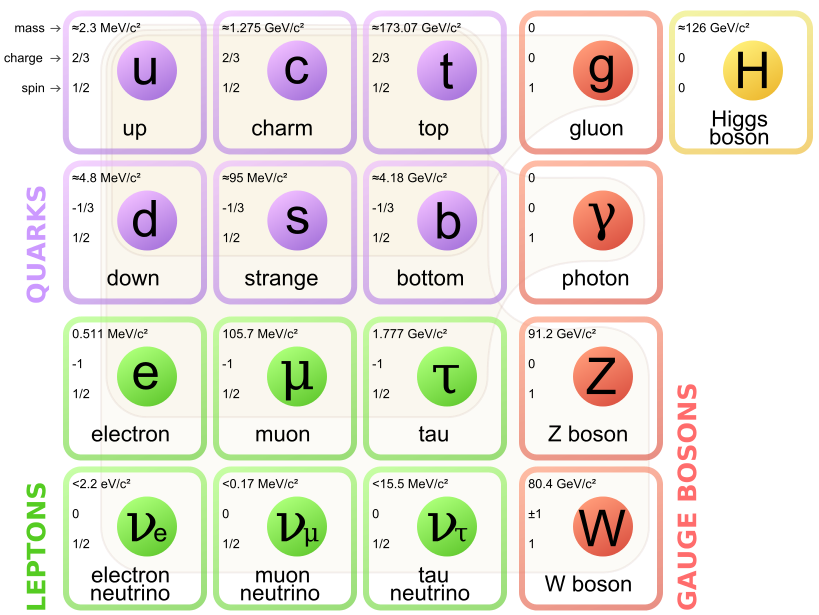
\includegraphics[width=\textwidth]{images/StandardModel}
\caption{The particles of the standard model.}
\end{figure}
\section{Symmetries}
In order to describe the interactions of elementary particles at high energies, one must introduce a quantum theory that is invariant under Lorentz transformations. These theories are typically described in terms of fields $\phi(x^0, x^1, x^2, x^3)$ and by specifying the \textit{Lagrangian Density} $\mathcal{L}(\phi, \frac{\partial \phi}{\partial x}, \frac{\partial \phi}{\partial t})$. \cite{tong} The Lagrangian density obeys the Euler-Lagrange equations:
\begin{equation}
\frac{\partial}{\partial X^{\mu}}(\frac{\partial \mathcal{L}}{\partial(\partial \phi/\partial X^{\mu})}) - \frac{\partial \mathcal{L}}{\partial \phi} = 0
\end{equation}
In the Standard Model, particles are represented by either vector or scalar fields, depending on their spins. The electron is represented by a field with two complex components at each point in space, while the spin-zero Higgs boson is represented by a scalar field. The scalar and vector fields in the Standard Model can often be transformed in such a way that the Lagrangian remains constant. These symmetries in the Standard Model can be expressed using the concept of a \textit{group}. The electromagnetic fields have symmetry according to the U(1) group, which is just the set of complex numbers with magnitude one, which can be expressed as $e^{i\theta}$, where $\theta$ takes any real value. Any two elements of U(1) multiplied together will give another element of U(1). For a scalar field, U(1) symmetry means that:
\begin{equation}
\phi = e^{i\theta}\phi
\end{equation}
for any $\theta$. When spin and color charge are taken into account, the overall symmetry of the Standard Model can be written as $SU(3) \times SU(2) \times U(1)$, where $SU(N)$ is the Special Unitary group, consisting of $N\times N$ unitary matrices with determinant one.\par

Substituting the Lagrangian for a system into the Euler-Lagrange equations gives the equations of motion of the system, from which the values of the fields at each point in space can be solved for. 

\section{The Large Hadron Collider}
In order to study the fundamental particles and their interactions, particle accelerators are typically used to accelerate particles to relativist energies and collide them, with detectors to observe the results of the collision. Since the particles are accelerated at energies close to the rest energies of particles such as the W and Z bosons, it is possible for these particles to be created during the collisions. The two main types of accelerators are linear and circular. Linear accelerators typically collide electrons and positrons together, while circular accelerators often use protons and anti-protons. This is due to \textit{Bremsstrahlung} radiation - photons that are emitted from accelerating charged particles. This radiation decreases according to the fourth power of the mass of the particle, so protons lose much less of their energy while accelerating around a loop. \par
The Large Hadron Collider (LHC) is a proton-antiproton collider located in Geneva, Switzerland. The LHC accelerates protons to relativistic energies of $7$ TeV, giving a total center of mass energy of $14$ TeV. 
\subsection{Coordinate System}
Coordinates inside the LHC are typically measured relative to the beam, with the z-axis pointing along the beamline, the positive y-axis pointing upward, and the positive x-axis pointing toward the center of the ring. The angle away from the beam axis is designated $\theta$, and the angle around the beam axis is called $\phi$. Rather than using $\theta$ directly, one typically uses the \textit{pseudorapidity} $\eta$, defined as: \cite{LHC2008}
\begin{equation} \label{eq:eta}
\eta = -ln\tan{\frac{\theta}{2}}
\end{equation}
In order to quantify the closeness of two particle tracks, one often uses $\Delta R$, the separation in eta-phi space:
\begin{equation}
\Delta R = \sqrt{(\phi_1 - \phi_2)^2 + (\eta_1 - \eta_2)^2}
\end{equation}
This can often be used to identify corresponding particles in two different data files that represent the same events.
\subsection{Luminosity}
The Luminosity of a collider is a measurement of how many particles travel through a unit surface area per time, and is useful for quantifying the statistical power that a collider can provide when searching for new particles. The total number of events expected after the collider has been running for some time is called the \textit{integrated luminosity} and is measured in inverse femtobarns ($fb^{-1}$). One can find the number of expected events for a certain process by multiplying the integrated luminosity by the cross-section of that process. In 2012, the LHC achieved $23 fb^{-1}$ worth of events, with luminosity at $10^{34}cm^{-2}s^{-1}$.\cite{LHC2008} \par
From 2015 to 2017, the LHC is expected to provide an additional $100 fb^{-1}$ of events, before being shut down for the "phase-I" upgrade, in which the luminosity will be increased to about $2\times 10^{34}cm^{-2}s^{-1}$ and the detectors will be upgraded to withstand the increased radiation from the higher luminosity. \cite{atlasupgrade} The third run of the detector will occur until about 2021, collecting $300 fb^{-1}$ of data. The final upgrade, phase-II, will happen in 2023, increasing the luminosity to $5\times 10^{34}cm^{-2}s^{-1}$. At this luminosity, an average of 140 collisions will happen per bunch-crossing, which poses significant challenges when trying to determine which vertex a particle came from. \cite{atlasupgrade}
\section{The ATLAS experiment}

\begin{figure}
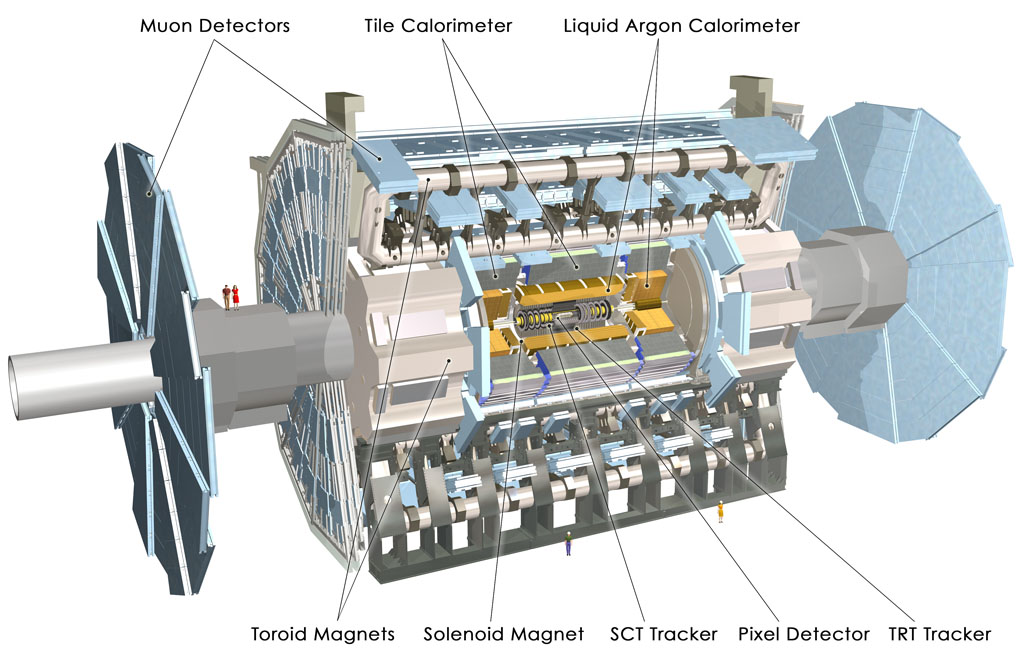
\includegraphics[width=\textwidth]{images/ATLAS_diagram}
\caption{Diagram of the ATLAS detector.\cite{ATLASDiagram}}
\end{figure}
ATLAS (A Toroidal LHC Apparatus) is one of the seven experiments located along the LHC ring. ATLAS is cylindrical, concentric rings of silicon pixel and strip detectors, calorimeters, and muon tracking chambers. The Inner Detector (ID) contains the first set of pixel and strip detectors. These are arranged in concentric cylinders around the beam-line, as well as in "end-caps" perpendicular to the beam-line. The barrel covers the region $|\eta| < 1.0$, and the endcaps cover $1.0 < |\eta| < 2.5$. The inner detector has a 2 Tesla magnetic field along the beam axis, which causes charged particles to curve. By using several layers of detectors, one can reconstruct the trajectory of the particle based on the point where it crosses each layer. The direction of the curvature of the particle gives its charge, and the magnitude of the curvature gives its momentum. \par
Outside the Inner Detector are the calorimeters, which measure the energies of charged particles and hadrons. Liquid Argon electromagnetic calorimeters are used to measure the energies of photons and electrons in the region $|\eta| < 3.2$. 

\section{Vector Boson Scattering}
Vector Boson scattering (VBS) is of particular interest because contributions from beyond-the-standard model theories would have a direct effect on the observed VBS cross sections at the LHC. \cite{atlasnote2012} The Higgs mechanism is the currently accepted theory for how WW scattering is unitarized. Without the Higgs mechanism, the WW scattering cross section does not approach zero at high-energies, which is necessary to keep the probability distributions normalized. \cite{atlasnote2012} \par
Previous work has pointed out that the leptonically-decaying channel of opposite-sign W-boson scattering (called leptonic WW scattering from now on) is a promising VBS interaction to study because the four-vectors of both W-bosons can be solved for, giving the WW invariant mass spectrum. \cite{atlasnote2012} Leptonic opposite-sign WW scattering is the following process:
\begin{equation} \label{eq:wwscattering}
p \bar{p} > W^+ W^- j j > q\bar{q} l^- \bar{v_l} jj
\end{equation}
\begin{equation}
p \bar{p} > W^+ W^- j j > q\bar{q} l^+ v_l jj
\end{equation}

where $p$ represents a proton, $\bar{p}$ represents an anti-proton, $W^{\pm}$ the W boson, $l$ either an electron or a muon, and $v_l$ the corresponding lepton neutrino. A Feynman diagram of the process is shown in figure \ref{fig:WWScatteringDiagram}.

\begin{figure}
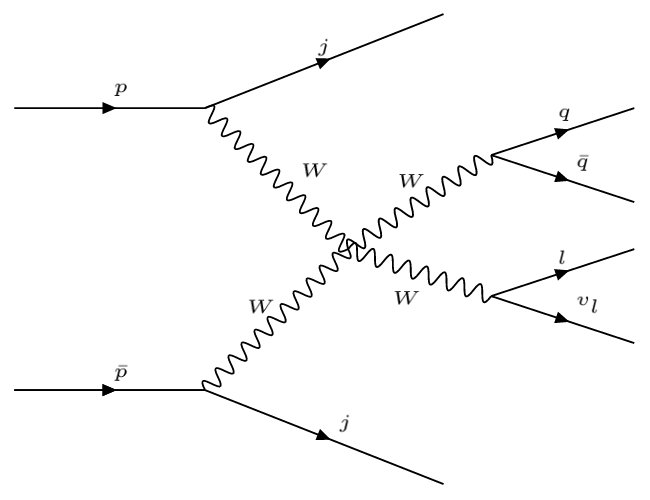
\includegraphics[width=8cm, height=8cm]{images/WWScatteringDiagram}
\caption{Feynman diagram of leptonically-decaying $W^{+}W^{-}$ scattering. The interaction between the two W bosons could be mediated by the Higgs or by other new physics.}
\label{fig:WWScatteringDiagram}
\end{figure}
According to \cite{atlasnote2012} leptonic WW scattering events can be identified by the presence of a lepton with $p_t > 60 GeV$, at least 25 GeV of missing transverse energy (representing the $p_t$ of the neutrino), two "tagging" jets in opposite $\eta$-hemispheres (the remnants of the protons), and one jet with mass between 60 GeV and 100 GeV (the "W-jet"). Although, the hadronically-decaying W actually decays to two jets, these two jets are close in $\Delta R$ and are reconstructed as one jet with mass close to the mass of the W. 

According to \cite{atlasnote2012}, the main obstacle to using leptonic WW scattering in searches for new physics is the $t\bar{t}$ background, which closely mimmicks the same final-state particles. They found that the W+3Jets and W+4Jets backgrounds were not significant.
\subsection{Effective Field Theories}
Assuming that the energy scale of new beyond-the-standard-model physics interactions is higher than the energy scale of the Large Hadron Collider, the best way to observe this new physics is to observe deviations from the Standard Model in interactions between known particles. If higher-energy interactions are occurring, they could be parameterized by adding terms to the Lagrangian that obey the Standard Model symmetries. These terms can be written as:
\begin{equation} \label{eq:effectivelagrangian}
\mathcal{L}_{eff} = \mathcal{L}_{SM} + \sum_{d>4}{\sum_{i}{\frac{\bar{c_i}}{\Lambda^{d-4}}O_i}}
\end{equation}

where $\Lambda$ is called the "scale" of the new physics - large $\Lambda$ means the effects only contribute at high energies. The $c_i$ are free parameters of the model. In this thesis, I will use simulated events based on these effective Lagrangians in order to come up with an estimate of how effective the HL-LHC will be when searching for new contributions to WW scattering.
\chapter{Methods}
\section{Monte-Carlo Event Simulation}
Since the Standard Model Lagrangian is extremely complex, computing the cross-sections of interactions exactly would be very difficult. In order to produce simulated events, one typically uses \textit{Monte Carlo} integration. This involves approximating the value of an integral by estimating the value of the integrand and multiplying by the length of the integration:
\begin{equation}
I = \int_{x_1}^{x_2}{f(x)dx} \approx (x_2 - x_1)\frac{1}{N}\sum_{i=0}^{N}{f(x_i)}
\end{equation}
where the $x_i$ are values between $x_1$ and $x_2$ drawn from a uniform distribution. \cite{MonteCarloHowTo} The variance of this estimate of the integral decreases as $\frac{1}{\sqrt{N}}$. 

The simulated WW scattering events were generated by VBFNLO, which uses Monte Carlo methods to calculate cross sections and particle trajectories. \cite{vbfnlo1}\cite{vbfnlo2} In addition to the Standard Model, VBFNLO can create simulated semi-leptonic WW scattering events under various effective operator Lagrangians. The events I use in this analysis have the dimension-6 operators enabled, and with several values of the scale factor $\Lambda$. The backgrounds used in this analysis are generated by MadGraph, another Monte-Carlo event generator. \cite{madgraph}\par
The parton-level events were then processed by Pythia 8.205, which hadronizes the parton-level particles. \cite{pythia}

\section{Reconstructing WW Invariant Mass}
Because the LHC accelerates protons to relativistic speeds, the kinematics of particle scattering and decay are governed by conservation of relativistic energy and momentum. Under the requirement of Lorentz invariance, the kinematics of a particle can be represented by the energy-momentum four-vector:
\begin{equation}p_{\mu} = (\frac{E}{c}, p_x, p_y, p_z) \end{equation}
where $p_x$, $p_y$, and $p_z$ are the relativistic momenta of the particle and $E$ is its total energy. The length of the energy-momentum four-vector (and all other Lorentz invariant four-vectors) is conserved under Lorentz transformations, where the length is defined by the inner product:
\begin{equation}p_{\mu} \cdot p_{\mu} = p_{\mu}p^{\mu} = -\frac{E^2}{c^2} + p_x^2 + p_y^2 + p_z^2 = -E^2 + |\vec{p}|^2 = -m^2\end{equation}
where $m$ is the called the invariant mass of the particle, and we have assumed that $c=1$ for convenience. In the last step we have used the relationship between relativistic momentum and energy:
\begin{equation}E^2 = p^2 + m^2 \end{equation}
For a particle decay, the four-vectors of the descending particles add to the four-vector of the original particle:
\begin{equation}p_{mother} = p_{daughter_1} + p_{daughter_2} + p_{daughter_3} + ...\end{equation}
For scattering, the four-vectors of the incoming particles add to the sum of the four-vectors of the outgoing particles:
\begin{equation}p_{incoming_1} + p_{incoming_2} = p_{outgoing_1} + p_{outgoing_2} \end{equation}
These two properties are very useful because they allow us to reconstruct the invariant masses of intermediate particles in an interaction by measuring the components of the four-vectors of the daughter particles. \par
 In WW scattering, both W bosons decay without being registered in any particle detectors, but their remnants (leptons and jets) can be detected and their momenta and energy can be measured. If the four-vectors of all daughter particles are known, the four-vectors of the W-bosons can be reconstructed.
In scattering experiments, the typical goal is to quantify the particle that mediates the scattering. Therefore, the invariant mass of the scattered particle pair is often of interest because peaks in the invariant mass spectrum would correspond to the mass of the particle mediating the interaction. 

In the case of semi-leptonic W+W- scattering, we wish to make a histogram of the invariant mass of the W-boson pair, starting with the four-vectors of the lepton, the hadronic jet, and the neutrino. The four-vectors of the lepton and the neutrino should add to the four-vector of the \textit{leptonic W}, and the four-vector of the hadronic jet should equal the four-vector of the \textit{hadronic W}. These two four-vectors can then be added to create the WW pair four-vector, from which the pair invariant mass can be calculated. Unfortunately, neutrinos are weakly interacting and their energy and momenta cannot be measured in any standard pixel/strip detector or calorimeter. Therefore, it is necessary to first reconstruct the neutrino's four-vector using the available information.

Fortunately, given the missing transverse energy for the event, it is possible to solve for the z-component of the neutrino's four-vector. The sum of the vectors for the neutrino and lepton is the four-vector of the leptonic W:
\begin{equation}W^{\mu} = l^{\mu} + n^{\mu} \end{equation}
Taking the magnitude of both sides:
\begin{equation}(W^{\mu})^2 = (l^{\mu} + n^{\mu})^2 \end{equation}
\begin{equation}W^{\mu}W_{\mu} = l^{\mu}l_{\mu} + 2l^{\mu}n_{\mu} + n^{\mu}n_{\mu} \end{equation}
The magnitude of a particle's energy-momentum four-vector is its invariant mass, so we can write:
\begin{equation}M_W^2 = M_l^2 + 2(E_nE_l - p_x^lp_x^n - p_y^lp_y^n - p_z^lp_z^n) + M_n^2 \end{equation}
where we have also used the definition of the energy-momentum four-vector to rewrite $l^{\mu}n_{\mu}$ in terms of the total energies of the particles and their relativistic momenta. Using the relation between relativistic momentum and energy, and assuming the neutrino is massless, we get:
\begin{equation}\frac{M_W^2 - M_l^2}{2} = E_l\sqrt{|p_t^n|^2 + (p_z^n)^2} - p_x^lp_x^n - p_y^lp_y^n - p_z^lp_z^n \end{equation}
where we have used the definition of transverse momentum, $|p_t|^2 = p_x^2 + p_y^2$. This gives a quadratic equation for $p_z^n$, the z-component of the neutrino's relativistic momentum. Using a computer algebra system, the solution can be found: \cite{moreno2009}
\begin{equation} \label{eq:pzsol}
p_z^n = \frac{-p_z^l(p_x^lE^{miss}_x + p_y^lE^{miss}_y + \frac{M_W^2 - M_l^2}{2}) \pm E_l\sqrt{(p_x^lE^{miss}_x + p_y^lE^{miss}_y + \frac{M_W^2 - M_l^2}{2})^2 + (E^{miss})^2(-E_l^2 + (p_z^l)^2)}}{E_l^2 - (p_z^l)^2}
\end{equation}
The lepton is typically detected in the tracker, so $p_x^l$, $p_y^l$ and $p_z^l$ are known. Since the neutrino is the only undetected final-state particle in the event, momentum conservation in the x-y plane makes it possible to estimate its $x$ and $y$ momentum components - they must be such that the total momentum in the x-y plane of all final-state particles adds to zero. Since the missing particle is assumed to be massless, this missing x-y momentum vector is often called "missing transverse energy": \cite{delphes}
\begin{equation} \label{eq:metdef}
\vec{E}^{miss} = -\sum{\vec{p}_t}
\end{equation}
Therefore, we have re-labeled $p_t^n$ to $\vec{E}^{miss}$ in equation \ref{eq:pzsol}. $E^{miss}$ has components 
\begin{equation}
\vec{p}_t^n \approx \vec{E}^{miss} = (E^{miss}_x, E^{miss}_y) = E^{miss}(\cos{\phi^m}, sin{\phi^m})
\end{equation}
where $\phi^m$ is the angle of the missing transverse energy vector $\vec{E}^{miss}$ in the $x$-$y$ plane. 

Equation \ref{eq:pzsol} works for computing the neutrino $p_z$ when the terms under the square-root add up to greater than zero. However, the discriminant could be negative, giving no solution for $p_z^n$. This can be resolved by changing the magnitude $E^{miss}$ such that the discriminant is zero, while preserving the angle of the missing transverse energy vector in the $x$-$y$ plane. This method is technically incorrect, since we are violating momentum conservation in the $x$-$y$ plane. However, by just changing $|E^{miss}|$ enough to make the discriminant zero, we are making the minimum error possible while still making the equation possible to solve. 
The condition for making the discriminant zero is:
\begin{equation}
(E^{miss}p_x^lcos{\phi^m} + E^{miss}p_y^lsin{\phi^m} + \frac{M_W^2 - M_l^2}{2})^2 + (E^{miss})^2(-E_l^2 + (p_z^l)^2) = 0 
\end{equation}
The solution for $E^{miss}$, which will be called $E'$, is: 
\begin{equation} \label{eq:metcorrection}
E' = \frac{-2\beta\alpha \pm \sqrt{4\beta^2\alpha^2 - 4\beta^2(\alpha^2 + (p_z^l)^2 - E_l^2)}}{2(\alpha^2 + (p_z^l)^2 - E_l^2)}
\end{equation}
\begin{equation} \alpha = p_x^l\cos{\phi^m} + p_y^l\sin{\phi^m} \end{equation}
\begin{equation} \beta = M_W^2 - M_l^2 \end{equation}
Once the value of $E'$ is known, it can be used as $E^{miss}$ in equation \ref{eq:pzsol} to find the neutrino $p_z$, where the discriminant is guaranteed to be zero. Another method for dealing with negative discriminants in equation \ref{eq:pzsol} that works better in practice is to fit the function
\begin{equation} \label{eq:metfit}
(E_x', E_y') = \frac{M_W^2 - M_l^2}{2[\sqrt{(p_t^l)^2 + M_l^2} - p_t^lcos{(\phi^n - \phi^l + \alpha)}]} (\cos{(\phi^n + \alpha)}, \sin{(\phi^n + \alpha)})
\end{equation}
so that $(E_x' - E^{miss}_x)^2$ and $(E_y' - E^{miss}_y)^2$ are minimum, by varying the parameter $\alpha$. \cite{nik}
\begin{figure}
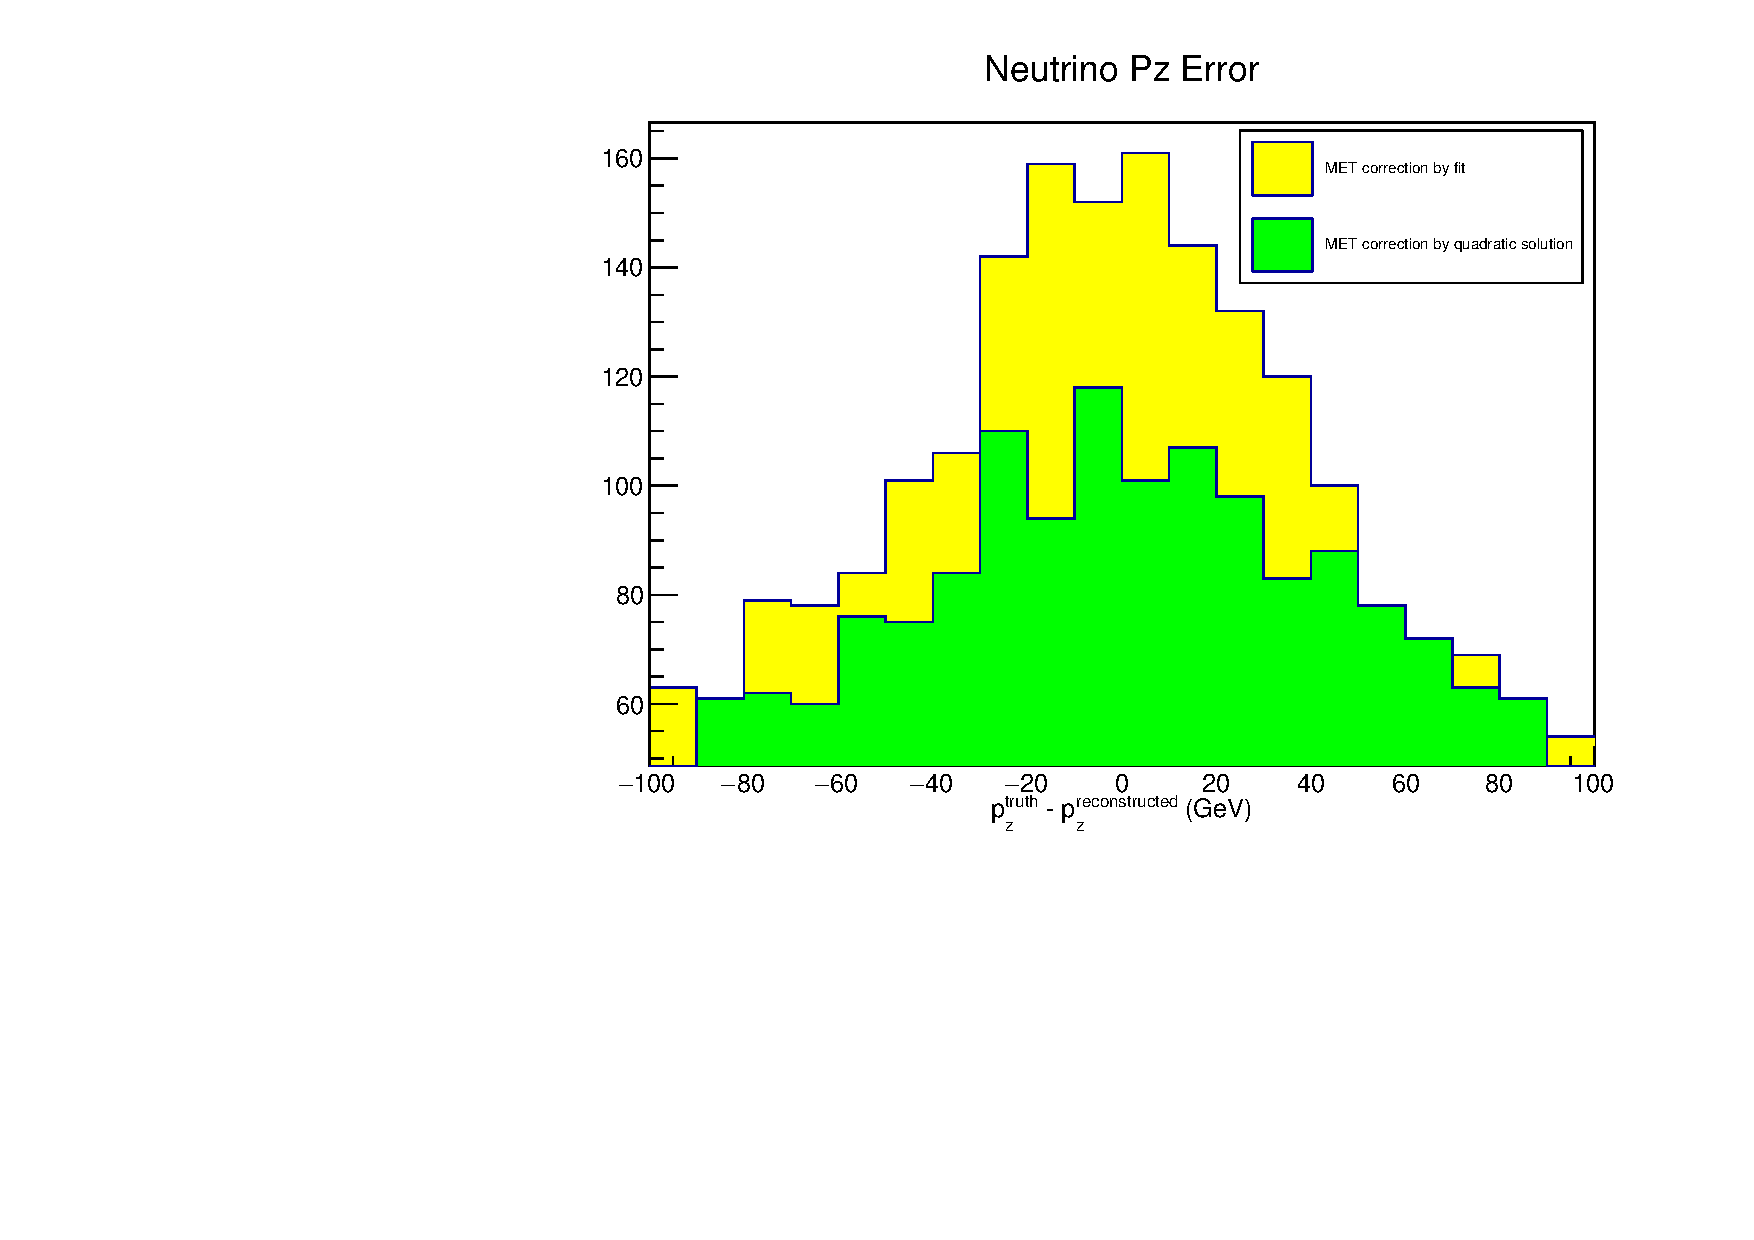
\includegraphics[height=8cm]{images/PzErrorMETCorrection}
\caption{The difference between the true neutrino $p_z$ and the corresponding $p_z$ estimated from equation \ref{eq:pzsol} with all discriminants set to zero by altering $E^{miss}$ according to equations \ref{eq:metcorrection} and \ref{eq:metfit}. The MET fitting method (equation \ref{eq:metfit}) gives more good $p_z$ values than the quadratic MET solution (equation \ref{eq:metcorrection}).}
\label{figure:pzerrormetcorrection}
\end{figure}
This fit gives a new missing transverse energy vector that makes the discriminant zero, while also staying close to the original missing transverse energy components. The new missing transverse energy can then be used in equation \ref{eq:pzsol} to find the neutrino $p_z$. This method allows both the direction and magnitude of the missing transverse energy vector to vary, in contrast to equation \ref{eq:metcorrection} which only varies the magnitude. The accuracy of the method in equation \ref{eq:metfit} compared to equation \ref{eq:metcorrection} is shown in figure \ref{figure:pzerrormetcorrection}. This fit method gets the neutrino $p_z$ close to the true value more frequently than the method in equation \ref{eq:metcorrection}, so we will use it from now on for resolving negative discriminants in equation \ref{eq:pzsol}. 

Figure \ref{figure:pzerrorbestmethods} shows the error when using equation \ref{eq:pzsol} to solve for $p_z$ and equation \ref{eq:metfit} to resolve negative discriminants. This is compared against equation \ref{eq:pzsol} by itself, with no attempt to resolve negative discriminants, in order to show that some additional neutrinos can be reconstructed accurately even when the discriminant is negative. It should be noted, however, that the chosen method also includes more bad neutrino reconstructions. 
\begin{figure}
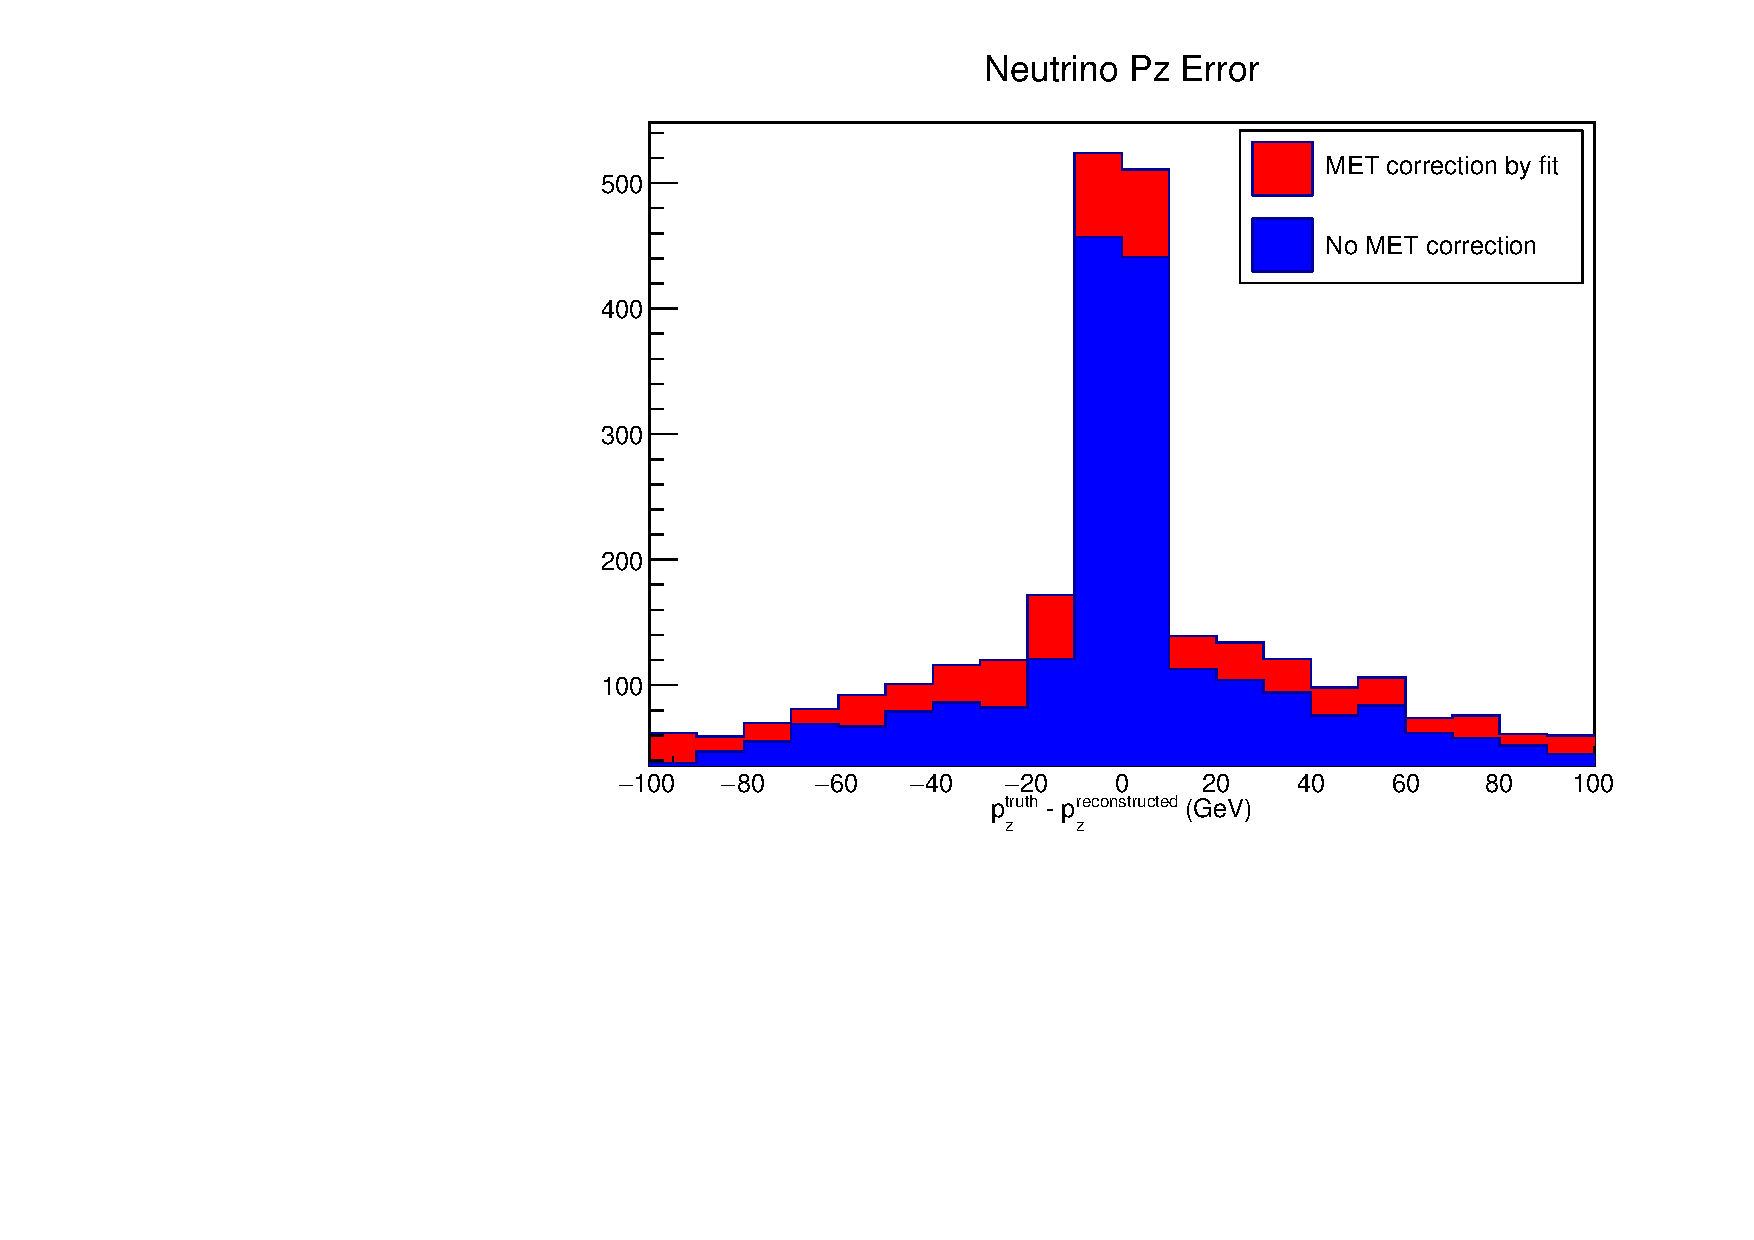
\includegraphics[height=8cm]{images/PzErrorBestMethods}
\caption{Difference between the true neutrino $p_z$ of parton-level WW scattering events and the corresponding neutrino $p_z$ estimated from equation \ref{eq:pzsol}. The error with missing transverse energy correction for negative discriminants is compared against the error with negative discriminant events thrown out.}
\label{figure:pzerrorbestmethods}
\end{figure}
\section{Detector Simulation}
The ATLAS pixel and strip detectors give measurements of the trajectories of charged particles in the ATLAS detector, and the calorimeters give measurements of their energies. These measurements are come with error that depends on the $\eta$ and $\phi$ position of the particle, and its energy and momentum. The Delphes 3.0 software package is used in this analysis to simulate detector uncertainty.

Delphes takes exact particle trajectories as input, and propagates them through the inner detector according to a magnetic field along the beam axis. \cite{delphes} This causes neutral particles to move in a straight line, while charged particles travel on a helical path. Each charged particle has some probability of being reconstructed as a track, which means that the direction of its momentum vector is recorded. The direction of the momentum vector is assumed to be perfectly accurate, but the magnitude of the transverse momentum is "smeared" according to Gaussian noise. Delphes assumes that the calorimeters are divided into Eta-Phi cells, and that the Electromagnetic Calorimeter (ECAL) is placed in front of the Hadronic Calorimeter (HCAL), such that each ECAL cell is in front of a corresponding HCAL cell. Electrons and photons deposit all of their energy in the ECAL by default, while heavier hadrons deposit a fraction of their energy in each calorimeter. Neutrons and muons don't deposit energy in the calorimeters. 
\subsection{Energy and Momentum Resolution}
Delphes parameterizes the energy and momentum resolution differently for each type of particle:
\begin{itemize}
\item Muons are not detected in the calorimeter, but the curvature of their tracks can be used to measure the muon $p_t$ accurately, which means the four-vector can be reconstructed without a measurement of the energy. Delphes randomly reconstructs the tracks of muons based on an efficiency formula defined in the parameter card, which depends on the $p_t$ and $\eta$ of the muon. The muon momentum four-vector is then smeared according to a Gaussian function with variance depending on $p_t$ and $\eta$.
\item Electrons are measured as tracks and their energy is deposited into the ECAL, which means their reconstruction efficiency depends on both the efficiency of the ECAL and the tracker. Delphes parameterizes this into a single efficiency function of $\eta$ and $E$. The energy resolution function also depends on both the ECAL and tracker resolution, and is also parameterized according to $\eta$ and $E$. 
\end{itemize}
Gaussian smearing of a measurement means that the measurement is drawn from a Gaussian distribution with the mean at the exact value:
\begin{equation} \label{eq:gausssmear}
P(X') = G(X_0, \sigma) = \frac{1}{\sqrt{2\pi}\sigma}\exp{[-\frac{(X' - X_0)^2}{\sigma^2}]}
\end{equation}
where $X_0$ is the exact value and $\sigma$ represents the resolution of the apparatus taking the measurement.

The default resolution functions for muon PT and electron energy are defined in the Delphes parameter card. For electron energy, the function is:
\begin{equation} \label{eq:DelphesEnergyRes}
\sigma_E = \sqrt{E^2a^2 + Eb^2 + c^2}
\end{equation}
The parameters $a$ and $b$ depend on both $\eta$ and $p_t$ and are shown in table \ref{tab:DelphesEnergyRes}.

\begin{table}[]
\centering
\caption{Default Delphes parameters for equation \ref{eq:DelphesEnergyRes}.}
\label{tab:DelphesEnergyRes}
\begin{tabular}{lllll}
$\eta$-condition & $E$-condition  & a    & b   &c     \\
$0 < |\eta| < 2.5$ & $0.1 < E < 25$   & 0.015 & 0.0 & 0.0 \\
$0 < |\eta| < 2.5$ & $E > 25$ & 0.005 & 0.05 & 0.25\\
$2.5 < |\eta| < 3.0$ & - & 0.005 & 0.05 & 0.25\\
$3.0 < |\eta| < 5.0$ & - & 0.107  & 0.208  & 0.0
\end{tabular}
\end{table}

For muons, Delphes uses a constant function for the momentum resolution:
\begin{equation} \label{eq:DelphesMuonRes}
\sigma_{p_t} = a
\end{equation}
where $a$ is given in table \ref{tab:DelphesMuonRes}.

\begin{table}[]
\centering
\caption{Default Delphes parameters for equation \ref{eq:DelphesMuonRes}.}
\label{tab:DelphesMuonRes}
\begin{tabular}{lll}
$\eta$-condition & $E$-condition  & a     \\
$0 < |\eta| < 1.5$ & $0.1 < p_t < 1.0$   & 0.03\\
$0 < |\eta| < 1.5$ & $1.0 < p_t < 5.0$ & 0.03\\
$0 < |\eta| < 1.5$ & $5 < p_t < 100$ & 0.04\\
$0 < |\eta| < 1.5$ & $p_t > 100$ & 0.07\\
$1.5 < |\eta| < 2.5$ & $0.1 < p_t < 1.0$ & 0.04\\
$1.5 < |\eta| < 2.5$ & $1.0 < p_t < 5.0$ & 0.04\\
$1.5 < |\eta| < 2.5$ & $5.0 < p_t < 100.0$ & 0.05\\
$1.5 < |\eta| < 2.5$ & $p_t > 100$ & 0.10
\end{tabular}
\end{table}

Delphes' default resolution functions are designed for the current ATLAS detector, but we are interested in simulating the planned phase-II upgrade, in which the structure of the detector will be different. New smearing functions have been published in \cite{ATLASElectronRes} and \cite{ATLASMuonRes}, based on simulations of the calorimeters and trackers in the proposed ATLAS detector. For electrons, the new function is:
\begin{equation} \label{eq:NewElectronRes}
\sigma_E = \sqrt{0.3^2 + 0.1^2E + 0.01^2E^2}, |\eta| < 1.4
\end{equation}
\begin{equation}
\sigma_E = \sqrt{0.3^2 + 0.15^2E + 0.015^2E^2}, |\eta| > 1.4
\end{equation}
The new muon momentum resolution functions are:
\begin{equation} \label{eq:sigmaID}
\sigma_{ID} = p_t \sqrt{a_1^2 + a_2^2p_t^2}
\end{equation}
\begin{equation} \label{eq:sigmaMS}
\sigma_{MS} = p_t\sqrt{(\frac{b_0}{p_t})^2 + b_1^2 + b_2^2p_t^2}
\end{equation}
\begin{equation} \label{eq:sigmaCB}
\sigma_{CB} = \frac{\sigma_{ID}\sigma_{MS}}{\sqrt{\sigma_{ID}^2 + \sigma_{MS}^2}}
\end{equation}
The functions $\sigma_{ID}$ and $\sigma_{MS}$ are the functions for the Inner Detector (ID) and Muon Spectrometer (MS) respectively. The function $\sigma_{CB}$ is a combination of those two functions, which behaves like each function for the $\eta$ and $p_t$ values where it is applicable. In order to correctly simulate the phase II detectors, I replaced the default Delphes functions in the parameter card with these new functions. \par
To check that Delphes was smearing the energies and momenta correctly, I created a set of parton-level events using MadGraph and then ran Delphes on them with the new parameter card. To check the electron smearing function, I created a set of $p p > Z > e+ e-$ events, and for the muon functions I created $p p > Z > \mu+ \mu-$ events. Then I compared the true electron energies from the parton-level file with the energies of the corresponding electrons in the Delphes output file, to find the amount each electron's energy had been smeared. I then created a \textit{profile plot} of the average difference from the true energy, as a function of the true energy. A profile plot (which is implemented in ROOT in the TProfile class) is used for showing the variance in a set of measurements, when the variance depends on the variable on the x-axis. In this case, we are dividing the electron energy axis into bins, and for each bin plotting the average deviation in electron energy from the true energy for the subset of electrons whose true energy falls into that bin. We can make a similar profile plot for muons to show their variance from the true $p_t$ as a function of the true $p_t$. \par
As a way of checking Delphes' internal implementation of smearing, I also performed the following procedure to generate simulated measurements smeared according to the new ATLAS functions:
\begin{itemize}
\item For each electron at parton level, get its energy $E$ and its $\eta$. 
\item Draw a value from a Gaussian distribution with mean $E$ and $\sigma$ determined by the ATLAS smearing function with the correct parameters for the electron's values of $p_t$ and $\eta$. 
\item Fill that value into a profile plot.
\end{itemize}

\begin{figure}
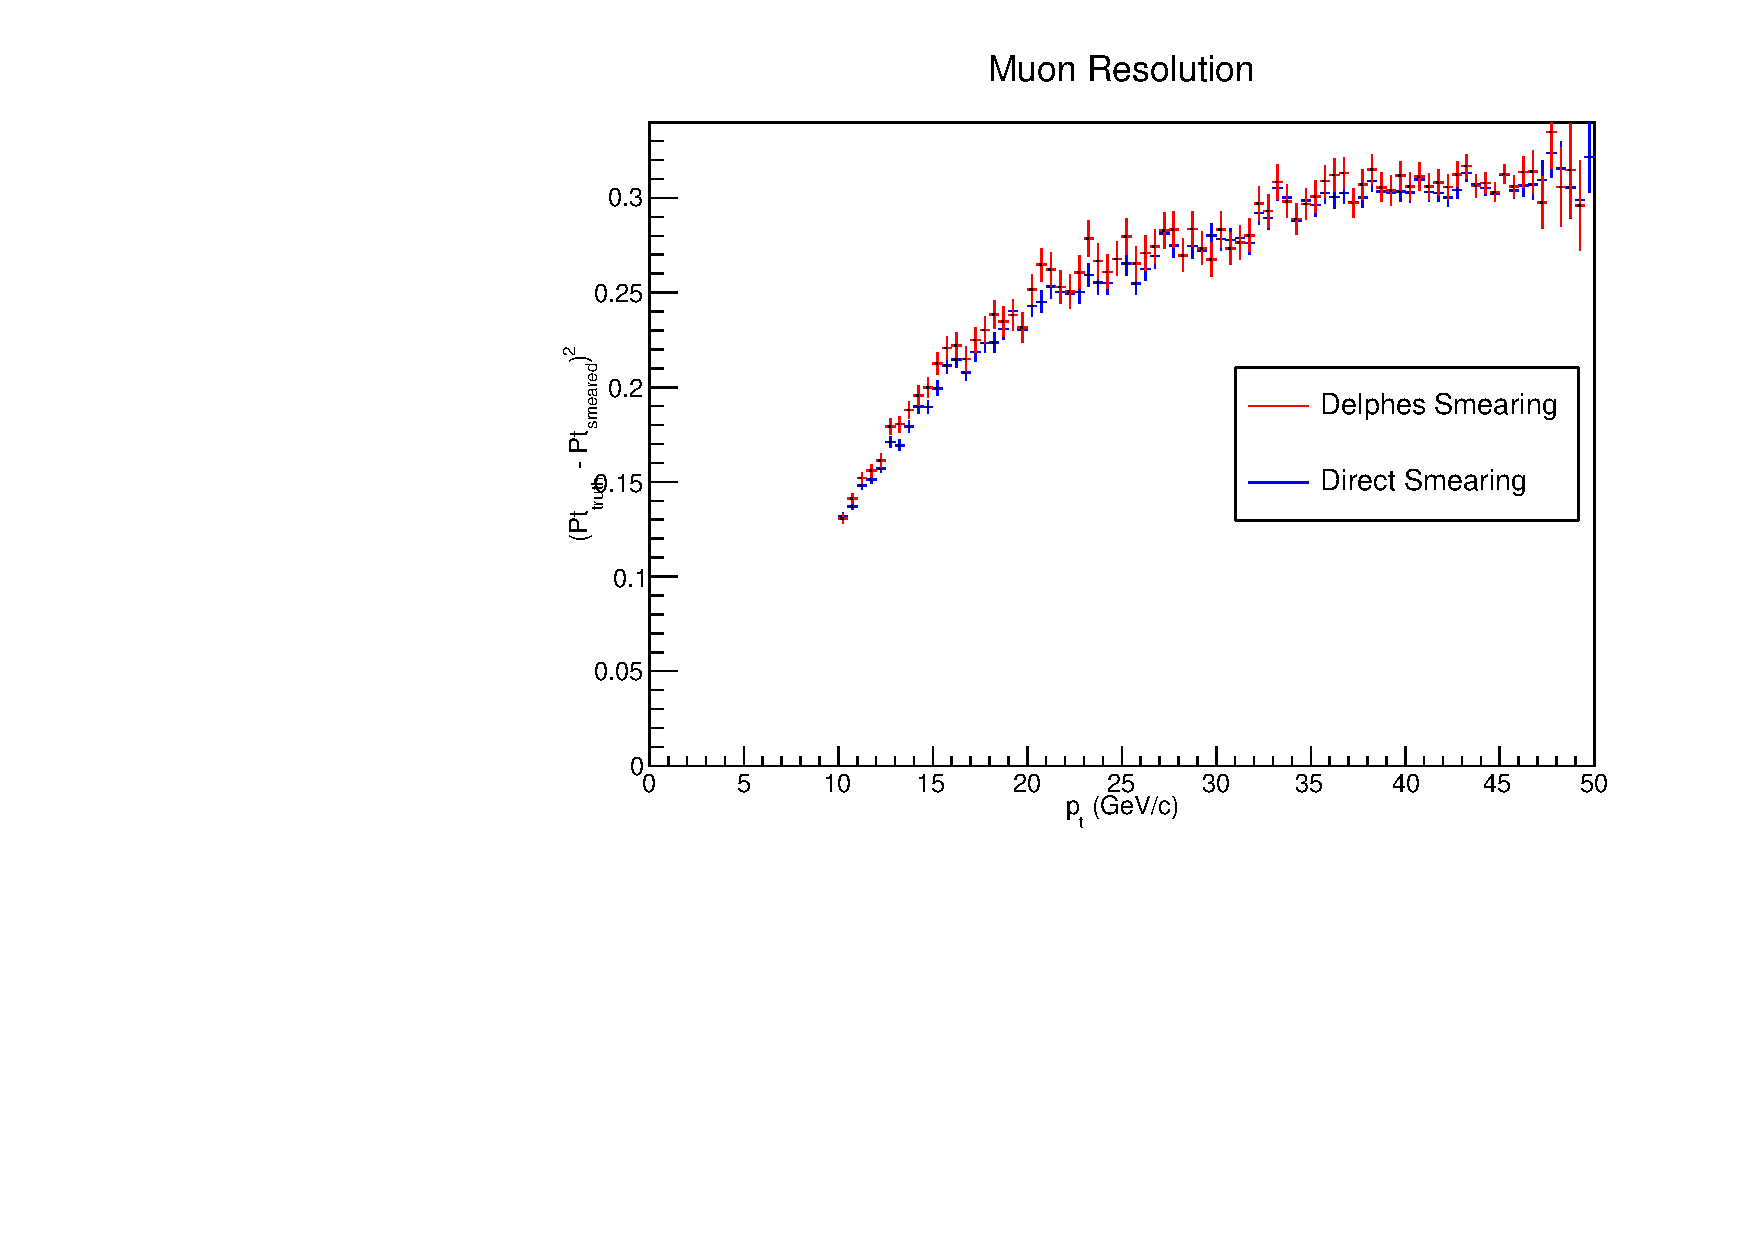
\includegraphics[height=8cm]{images/MSSmearing}
\caption{Profile plot of Muon smearing with the MS smearing function.}
\label{fig:SigmaMS}
\end{figure}
\begin{figure} 
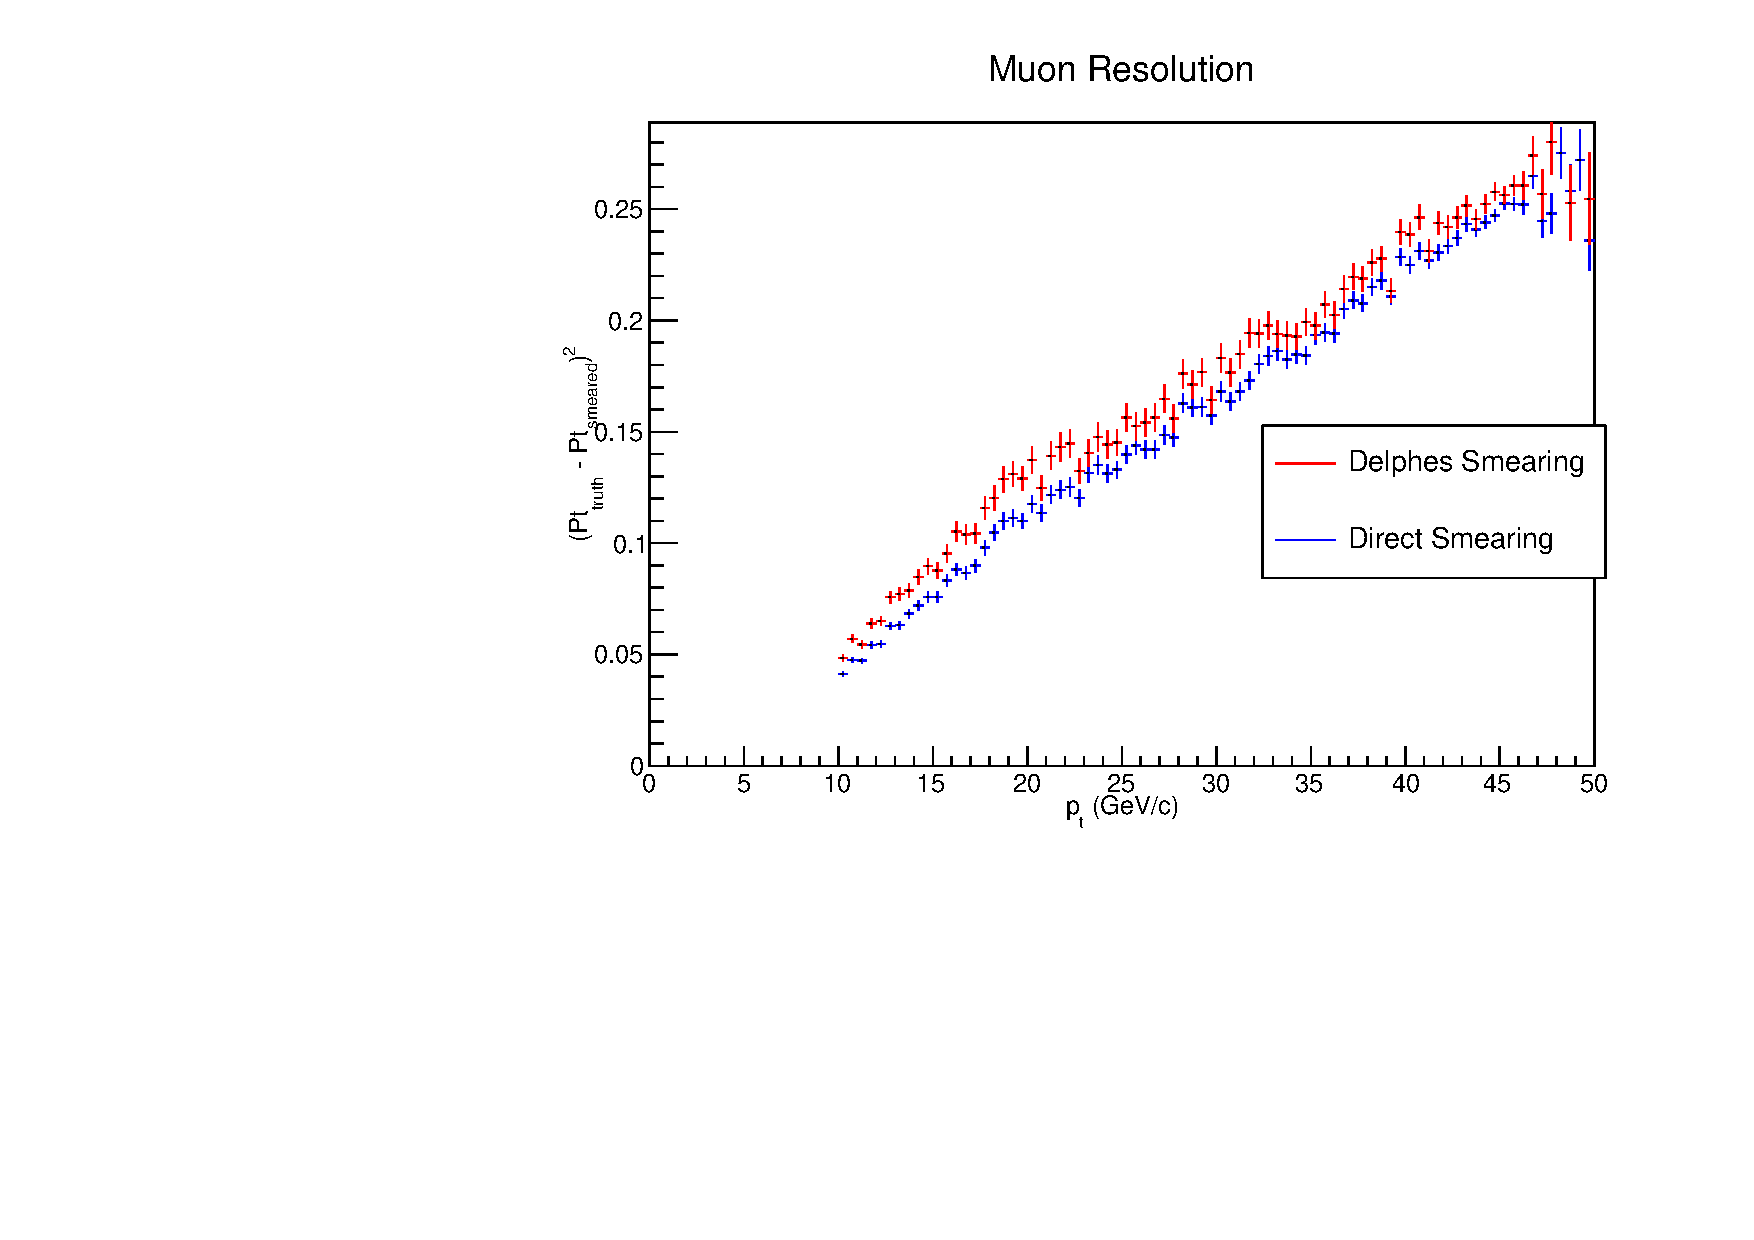
\includegraphics[height=8cm]{images/IDSmearing}
\caption{Profile plots of the muon $p_t$ difference between the smeared and unsmeared muons in a set of $Z > \mu+ \mu-$ events.}
\label{fig:SigmaID}
\end{figure}
\begin{figure}
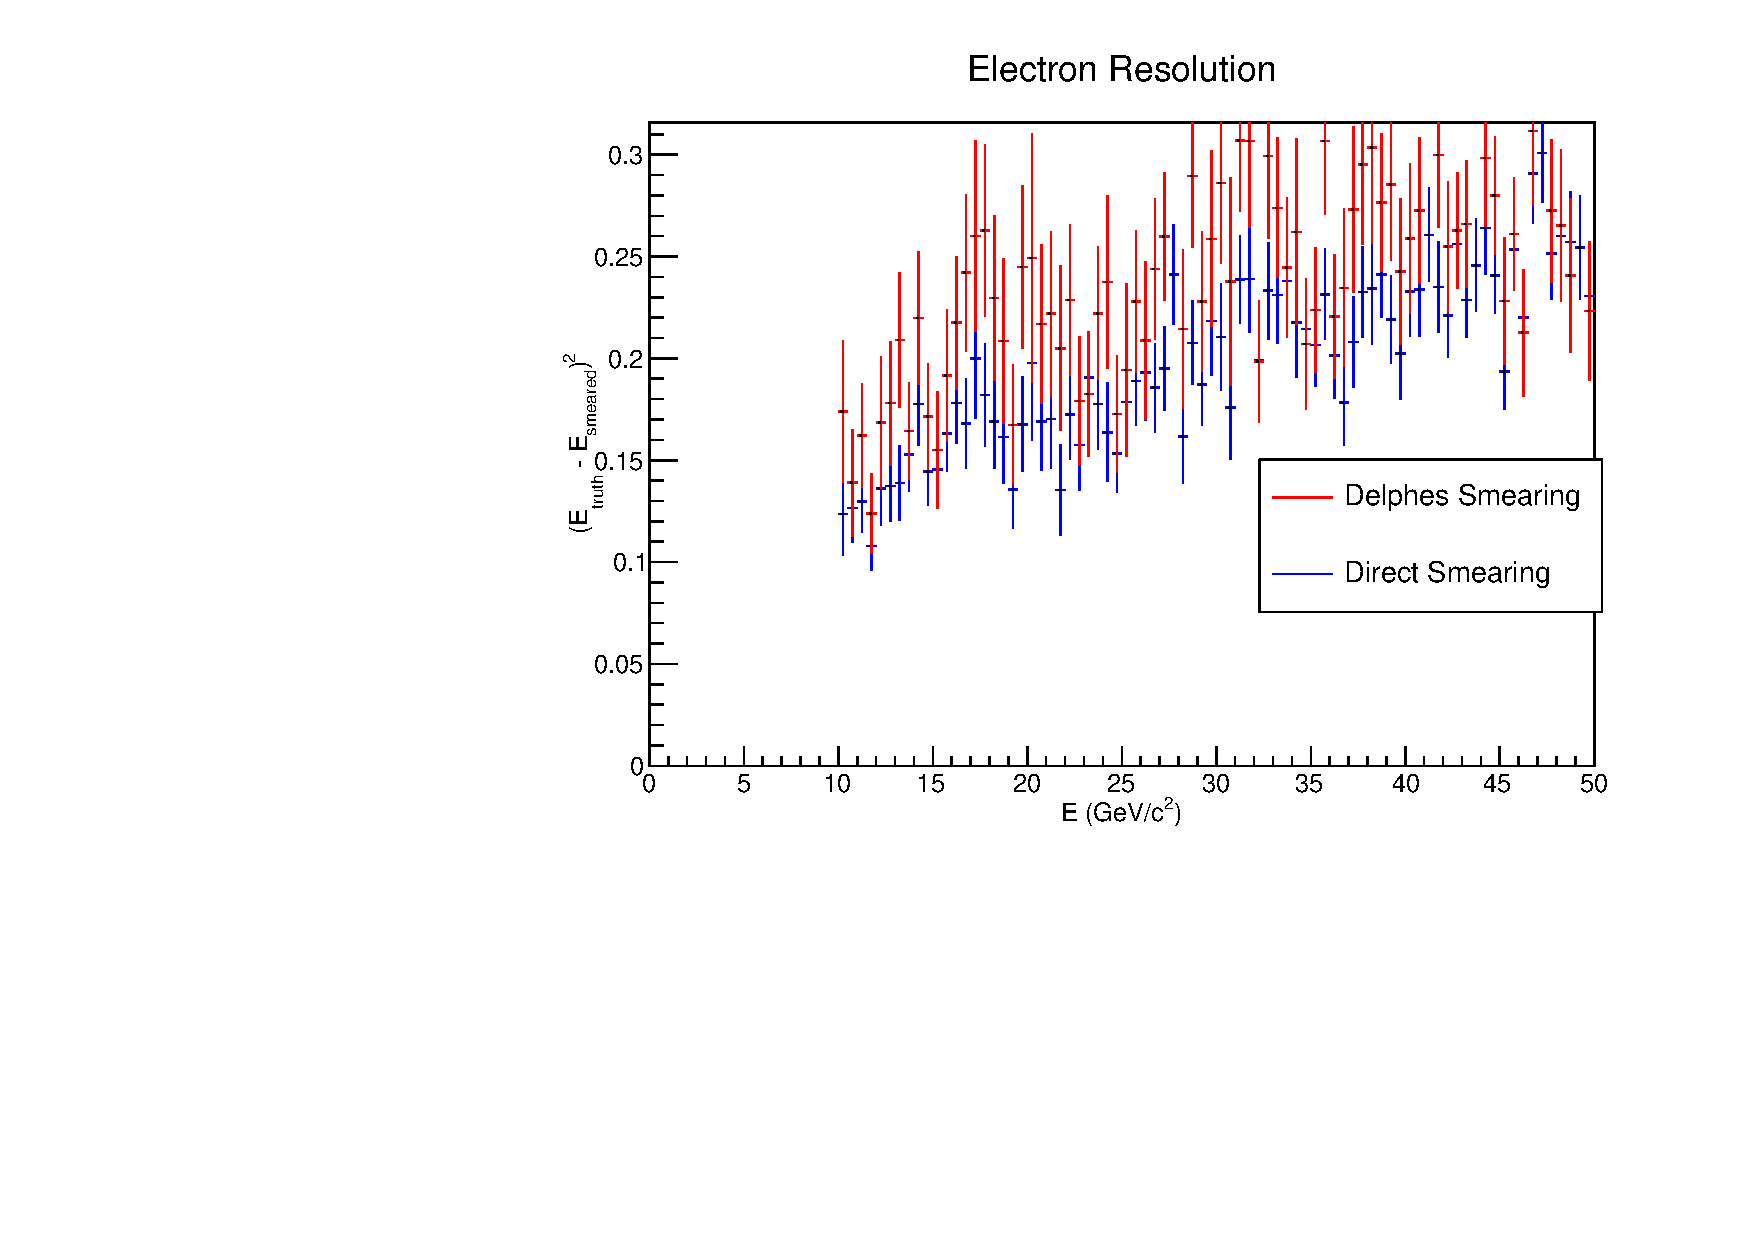
\includegraphics[height=8cm]{images/ElectronSmearing}
\caption{Electron energy resolution with the smearing functions proposed in \cite{ATLASElectronRes}}
\label{fig:SigmaElectron}
\end{figure}
A similar procedure applies for generating simulated muon $p_t$ measurements. Figure \ref{fig:SigmaMS} shows the profile plot of the muon $p_t$ deviation for Delphes and for the above procedure, with the $\sigma_{MS}$ resolution function, and figure \ref{fig:SigmaID} shows the same for $\sigma_{ID}$. Delphes' resolution agrees very well with the direct smearing procedure, so I will claim that the smearing is being done correctly.


\section{Event Selection}
\subsection{Tagging Jet Classifier}
Since the WW scattering events we wish to observe are primarily characterized by two far-forward (high-$\eta$) jets, it is necessary to identify these two jets before attempting to reconstruct the WW pair mass. The main obstacle to distinguishing these tagging jets from other jets in an event is pileup. The LHC collides bunches of protons and anti-protons with each other, with each bunch-crossing resulting in multiple proton-antiproton collisions. The expected number of collisions is given by: \cite{ATLASJVF}
\begin{equation}
<\mu> = \frac{L\sigma_{pp}}{N_{bunch}f_{LHC}} 
\end{equation}
where $\sigma_{pp}$ is the cross section of proton-proton interactions, $L$ is the luminosity of the LHC, $N_{bunch}$ is the number of electrons per bunch, and $f_{LHF}$ is the frequency of the LHC - the number of bunches passing a given point per second.
The higher the luminosity of the accelerator, the more collisions will occur each time the bunches cross. With many vertices in each bunch-crossing, it becomes difficult to determine which vertex a detected particle originated from. Jets are particularly difficult to associate with a vertex because they are actually groups of particles. Once tracks have been clustered into jets (usually by the Anti-KT algorithm), a quantity called the \textit{Jet Vertex Fraction} (JVF) can be defined:
\begin{equation}
JVF = \frac{\sum_{i}{p_t(PV_\alpha, i)}}{\sum_{j}\sum_{i}{p_t(PV_j, i)}}
\end{equation}
where $j$ ranges over all primary vertices and $i$ ranges over all particles whose tracks originate from a particular primary vertex. The JVF is a measure of the fraction of the transverse momentum of a jet that originated from primary vertex $\alpha$. If the JVF is close to zero, most of the transverse momentum in the jet comes from vertices other than $\alpha$. If it's close to one, most of the transverse momentum did originate from that vertex. Therefore, the JVF is a measurement of the likelihood that a jet came from a pileup vertex, rather than the primary vertex in the event. Usually the primary vertex is determined by the tracks of the other particles, such as leptons.

In addition to the JVF, figure \ref{fig:jetvars} shows several variables that have significantly different distributions for tagging jets than for pileup jets. We would like to use all of these variables simultaneously for each candidate jet to decide whether it is pileup or tagging.

One method of classifying jets would be to simply require the JVF to be above a certain threshold - this is called a \textit{cut}. One could also make cuts on other variables like jet $p_t$, jet $\eta$, or jet mass. The problem with this method is that it might be overly harsh in rejecting *all* jets that fail any of the cuts. It would be better to consider all variables simultaneously when classifying each jet. The best way to do this is through \textit{machine learning} (ML) classification.

\begin{figure} \label{fig:jetvars}
	\centering
	\begin{subfigure}[b]{0.4\textwidth}
    	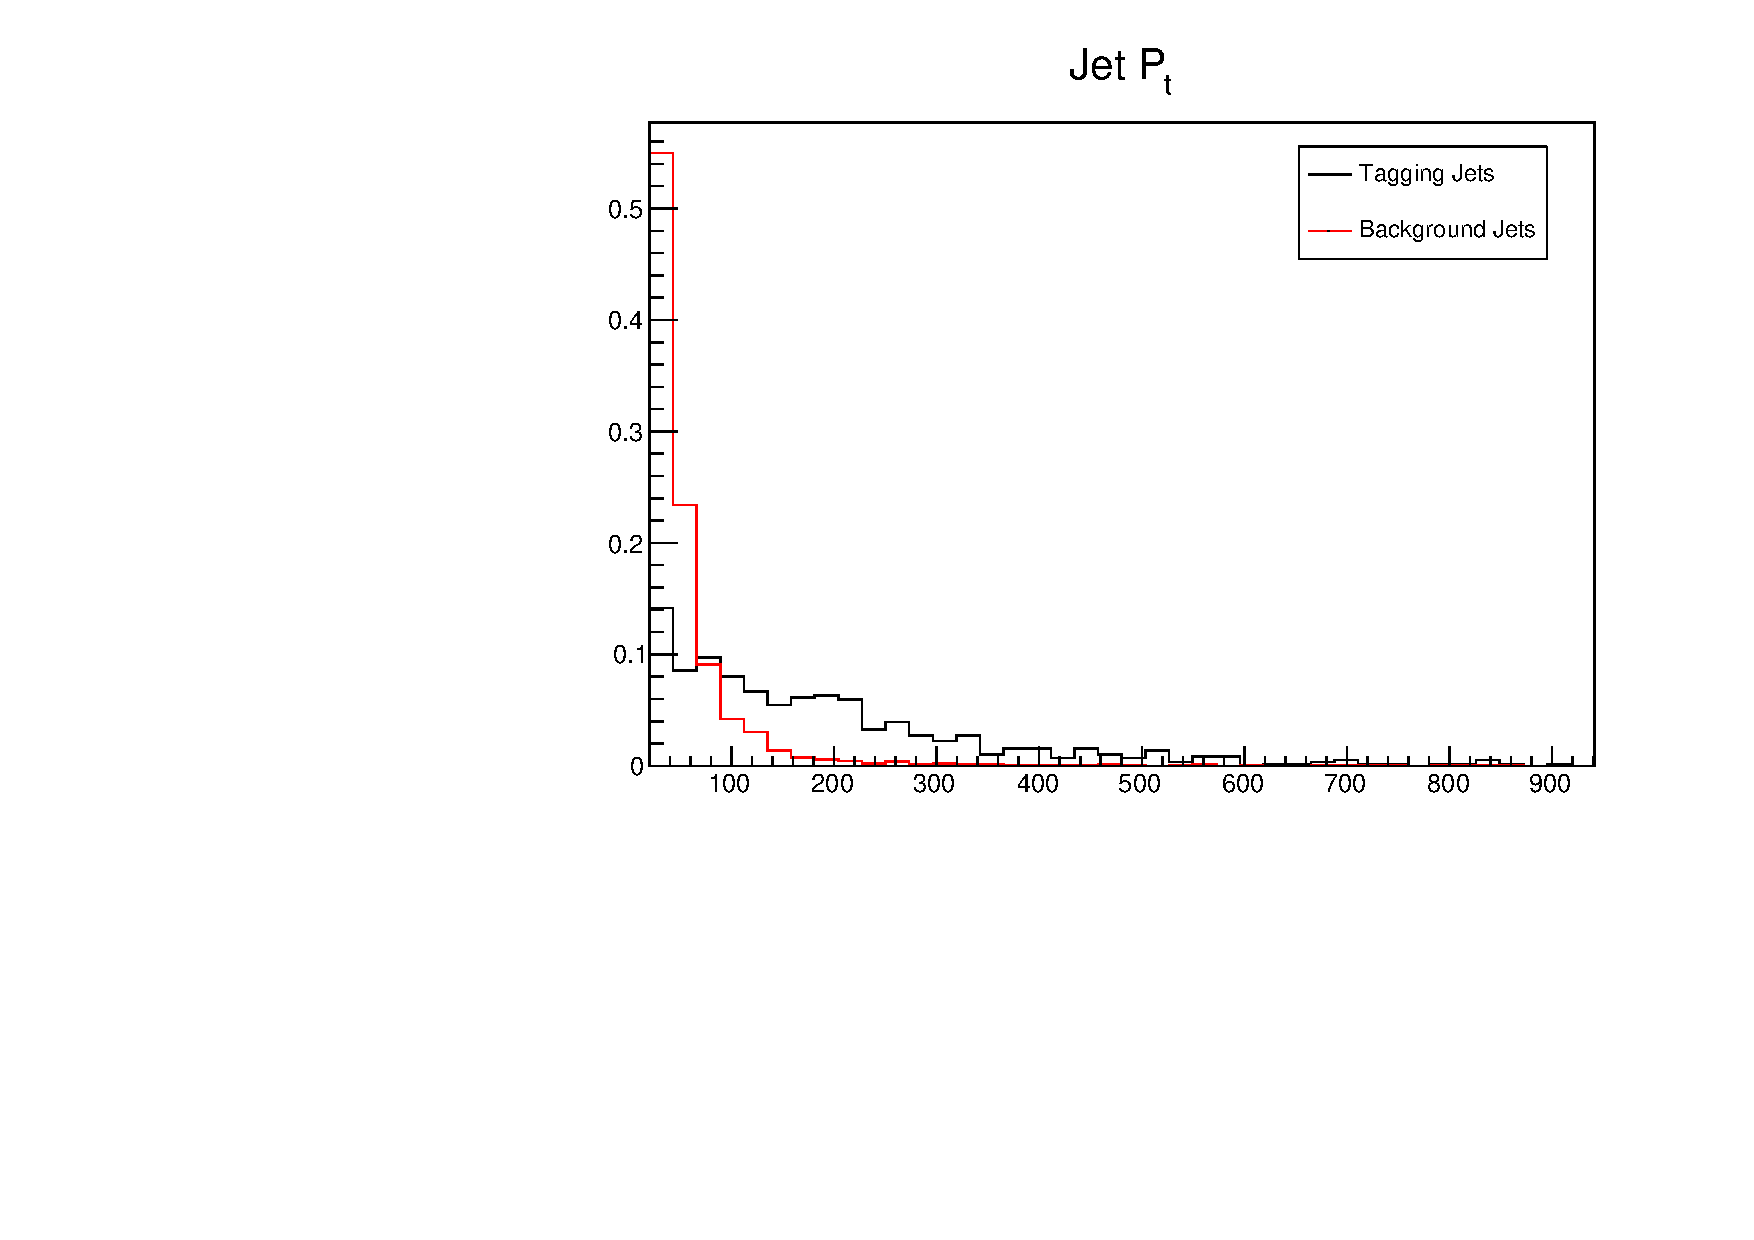
\includegraphics[width=\textwidth]{images/JetPT}
        \subcaption{Jet transverse momentum}
    \end{subfigure}
    \begin{subfigure}[b]{0.4\textwidth}
    	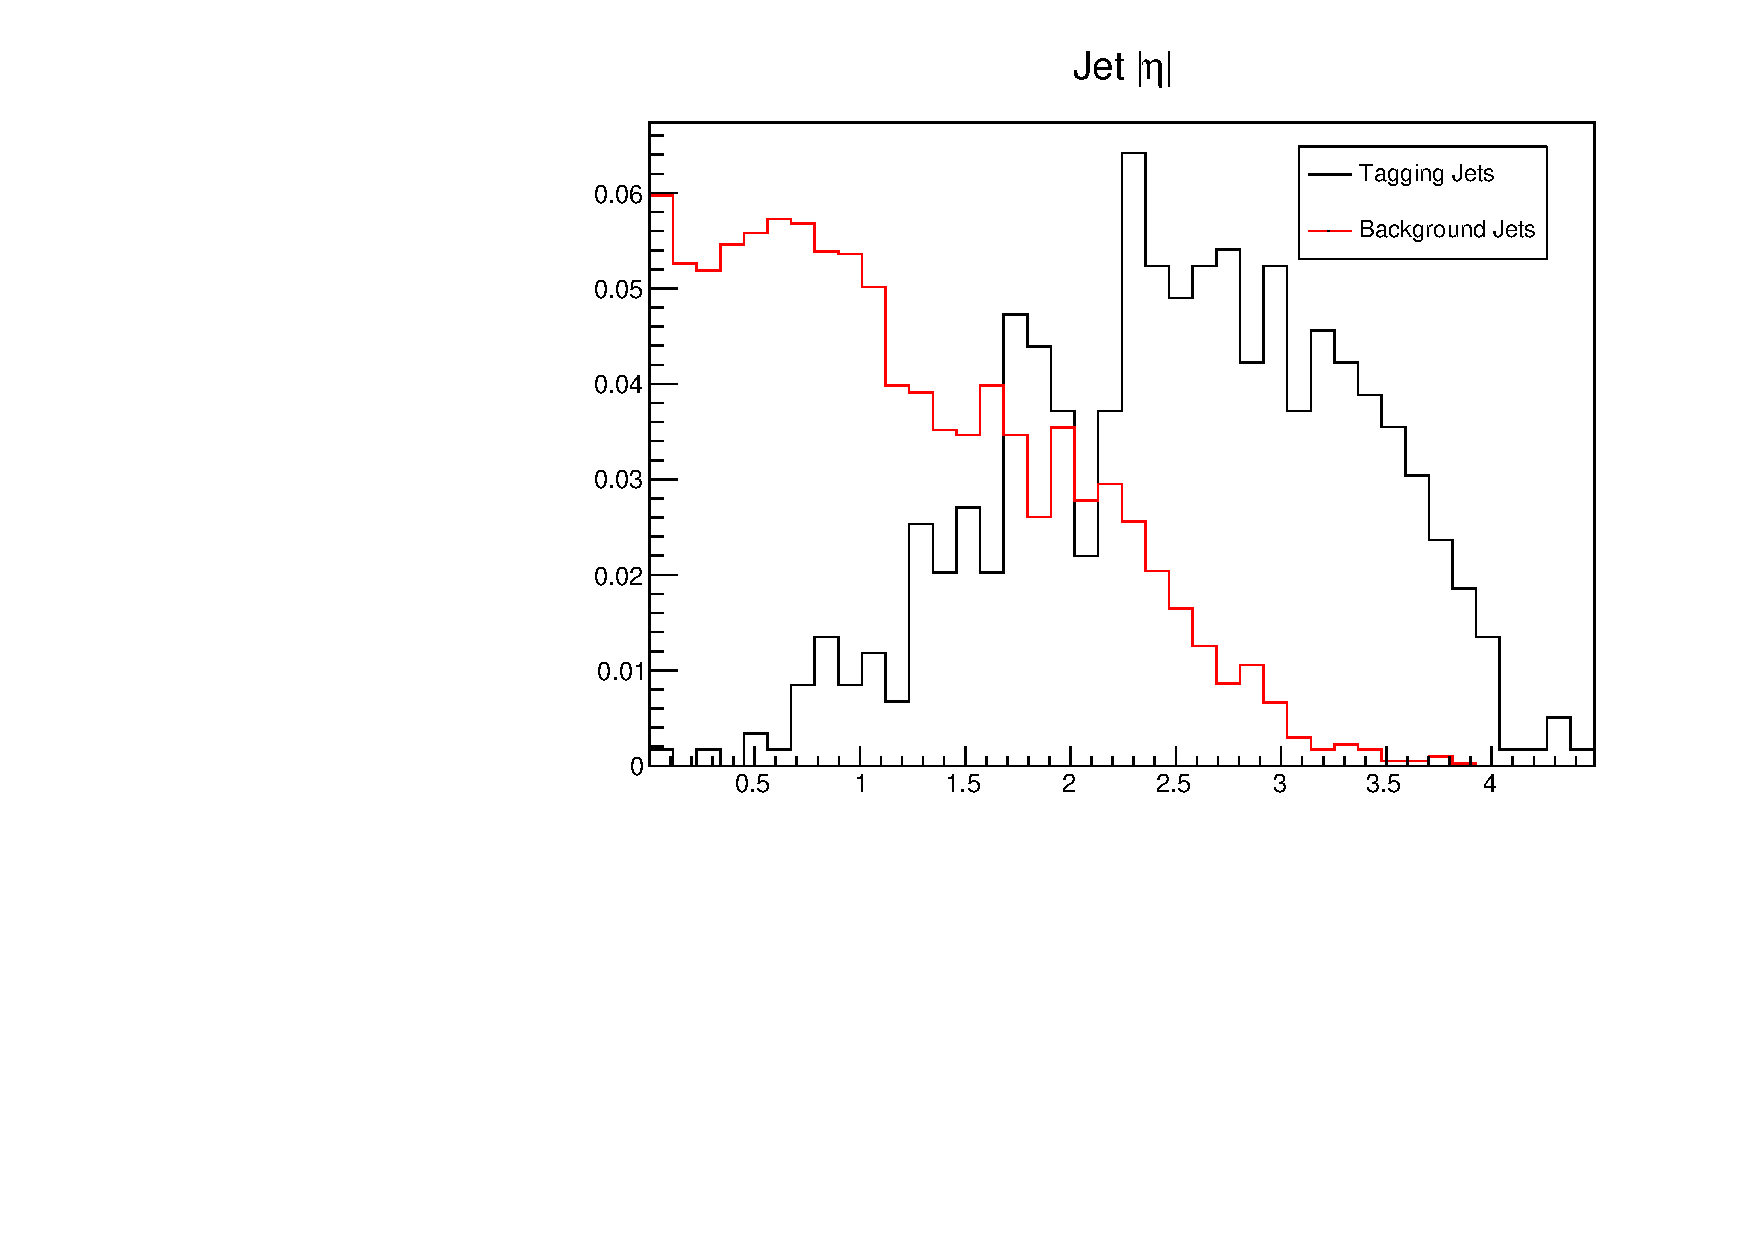
\includegraphics[width=\textwidth]{images/JetAbsEta}
        \subcaption{Jet $|\eta|$}
    \end{subfigure}
    \begin{subfigure}[b]{0.4\textwidth}
    	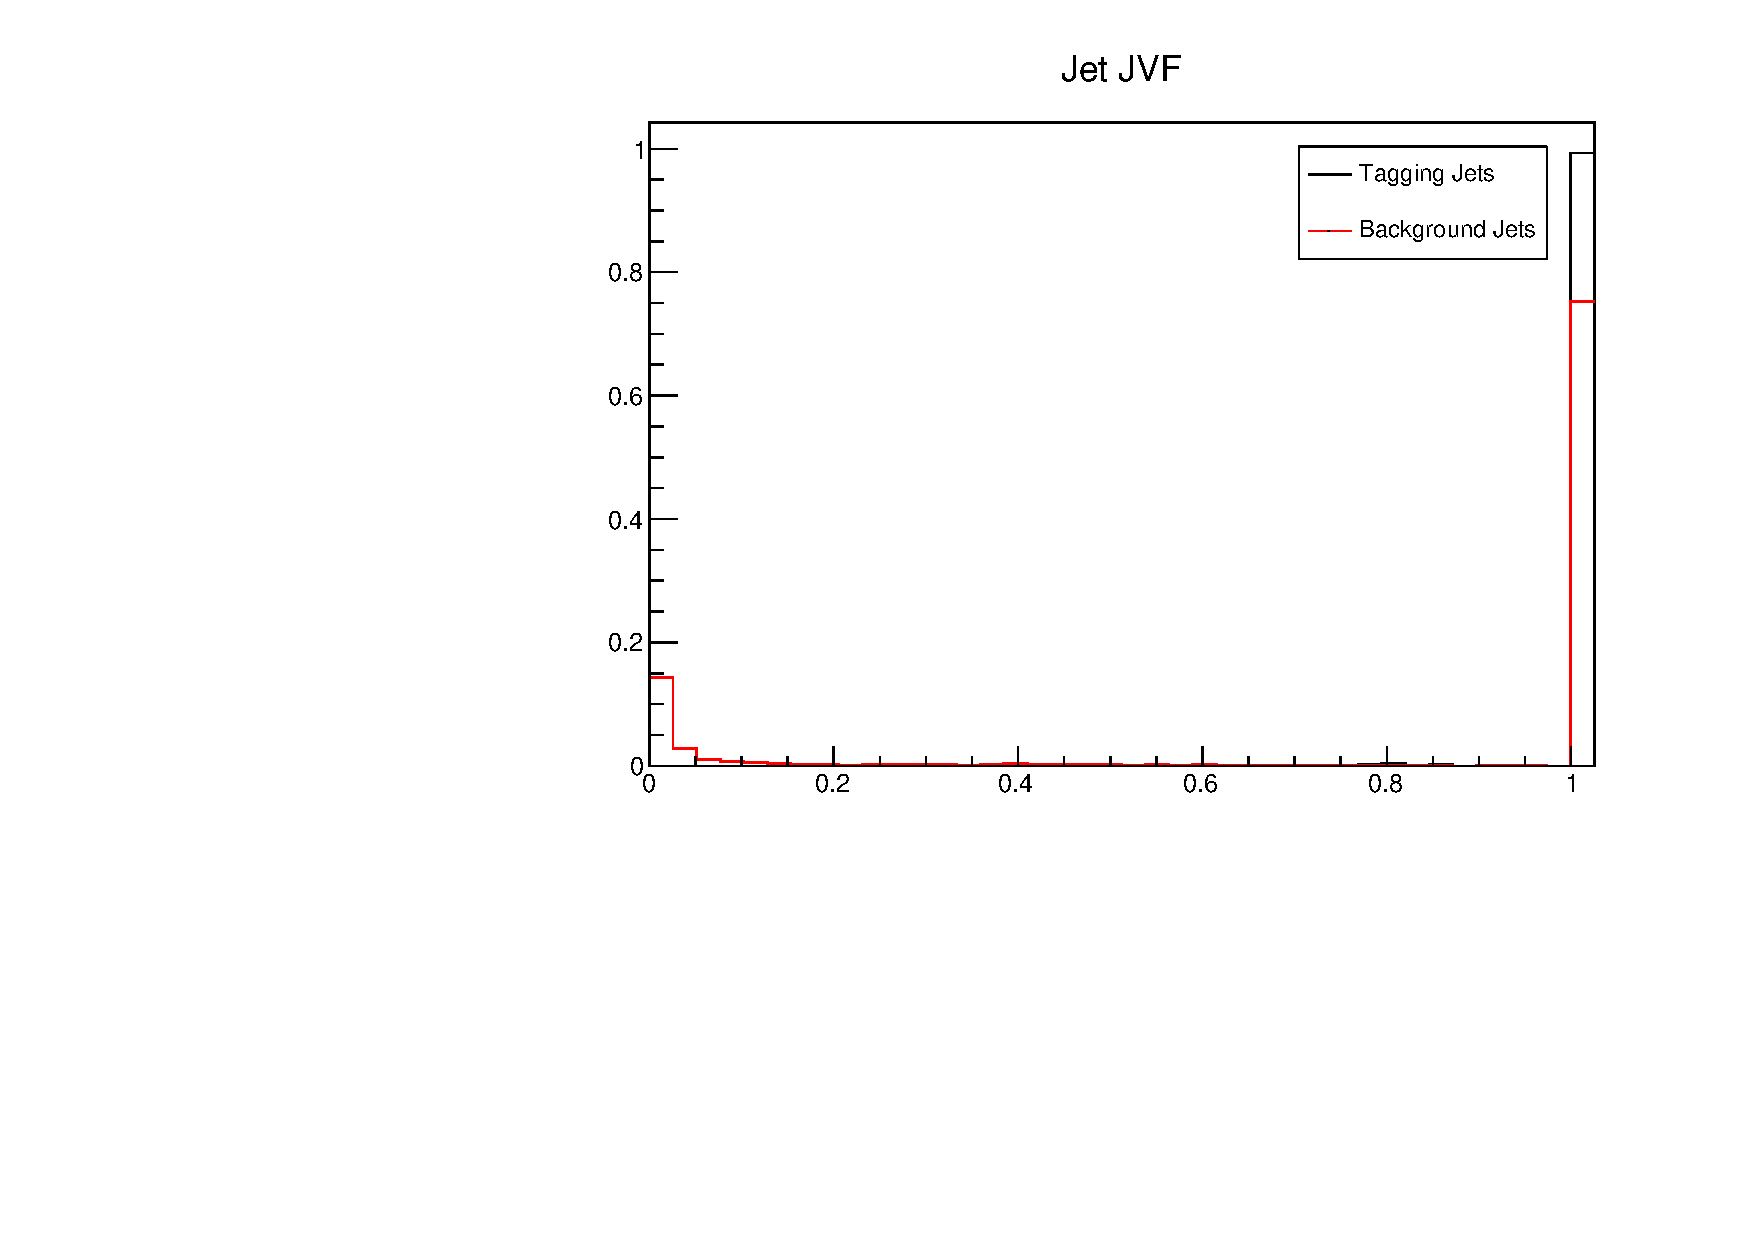
\includegraphics[width=\textwidth]{images/JetJVF}
        \subcaption{Jet Vertex Fraction}
    \end{subfigure}
    \caption{Normalized distributions of jet $|\eta|$, $p_t$, and JVF for a set of tagging jets and a set of background jets. Variables whose distributions differ between the two categories of jets are useful for classification.}
    \label{fig:jetvars}
\end{figure}

Using machine learning algorithms, it is possible to "train" a classifier to sort a set of samples (in this case, jets) into two or more categories. The most basic classifier would be a linear function of the set of variables we are using for classification:
\begin{equation}
y = w_1x_1 + w_2x_2 + w_3x_3 + ...
\end{equation}
where ${x_i}$ are a set of variables, ${w_i}$ are the weights given to each of those variables, and $y$ is the $response$ of the classifier for a particular sample. The response is a number between zero and one that represents the category the sample has been classified into. This linear classifier could be trained by using samples whose classification are known. This is called a "training set". Over this training set, the weights could be chosen such that they minimize the quantity
\begin{equation}
\sum_i(y_i - y_i^{truth})^2 + |w|^2
\end{equation}
, where $y_i^{truth}$ is the true category of jet $i$ and $y_i$ is the classifier response. The second term is the norm of the weight vector - including this term helps prevent the weights from becoming arbitrarily large and "overfitting" to the training set. \par
Linear classifiers are effective for some problems, but there are more complicated classifiers that use non-linear functions of the input variables, and these are often more effective. For identifying the tagging jets, we will use a method called \textit{Boosted Decision Tree} \cite{BDT}, which was found to be effective for this problem in prior work by Niklas Garner \cite{nik}. However, most classifier algorithms give very similar results - the most important step is choosing features that effectively separate the two classification categories. \par
In order to train the tagging jet classifier, we need a set of known tagging jets and a set of known pileup jets, over which the classifier training algorithm will optimize the parameters of the BDT such that the training samples are classified correctly. We can obtain this training set from a set of WW scattering events produced by VBFNLO/MadGraph/Delphes, by checking whether each jet in the Delphes-level events corresponds to a jet in the parton-level file. If an event has two jets in opposite $\eta$ hemispheres that can be matched to parton-level quarks, those two jets are considered tagging jets. All other jets are assumed to be pileup. \par

To train and test the BDT, I created a set of 1184 known tagging jets and 8134 known pileup jets from 1000 WW scattering events. I then used TMVA to train a BDT on half of this training set, and test the classification efficiency on the other half. The complete set of variables used were:
\begin{itemize}
\item Jet $|\eta|$
\item Jet $p_t$
\item Jet energy
\item Jet mass
\item Jet JVF
\end{itemize}
The efficiency (percentage of jets that are classified as tagging) over the test set is shown in figure \ref{fig:jetbdteff}.
\begin{figure}
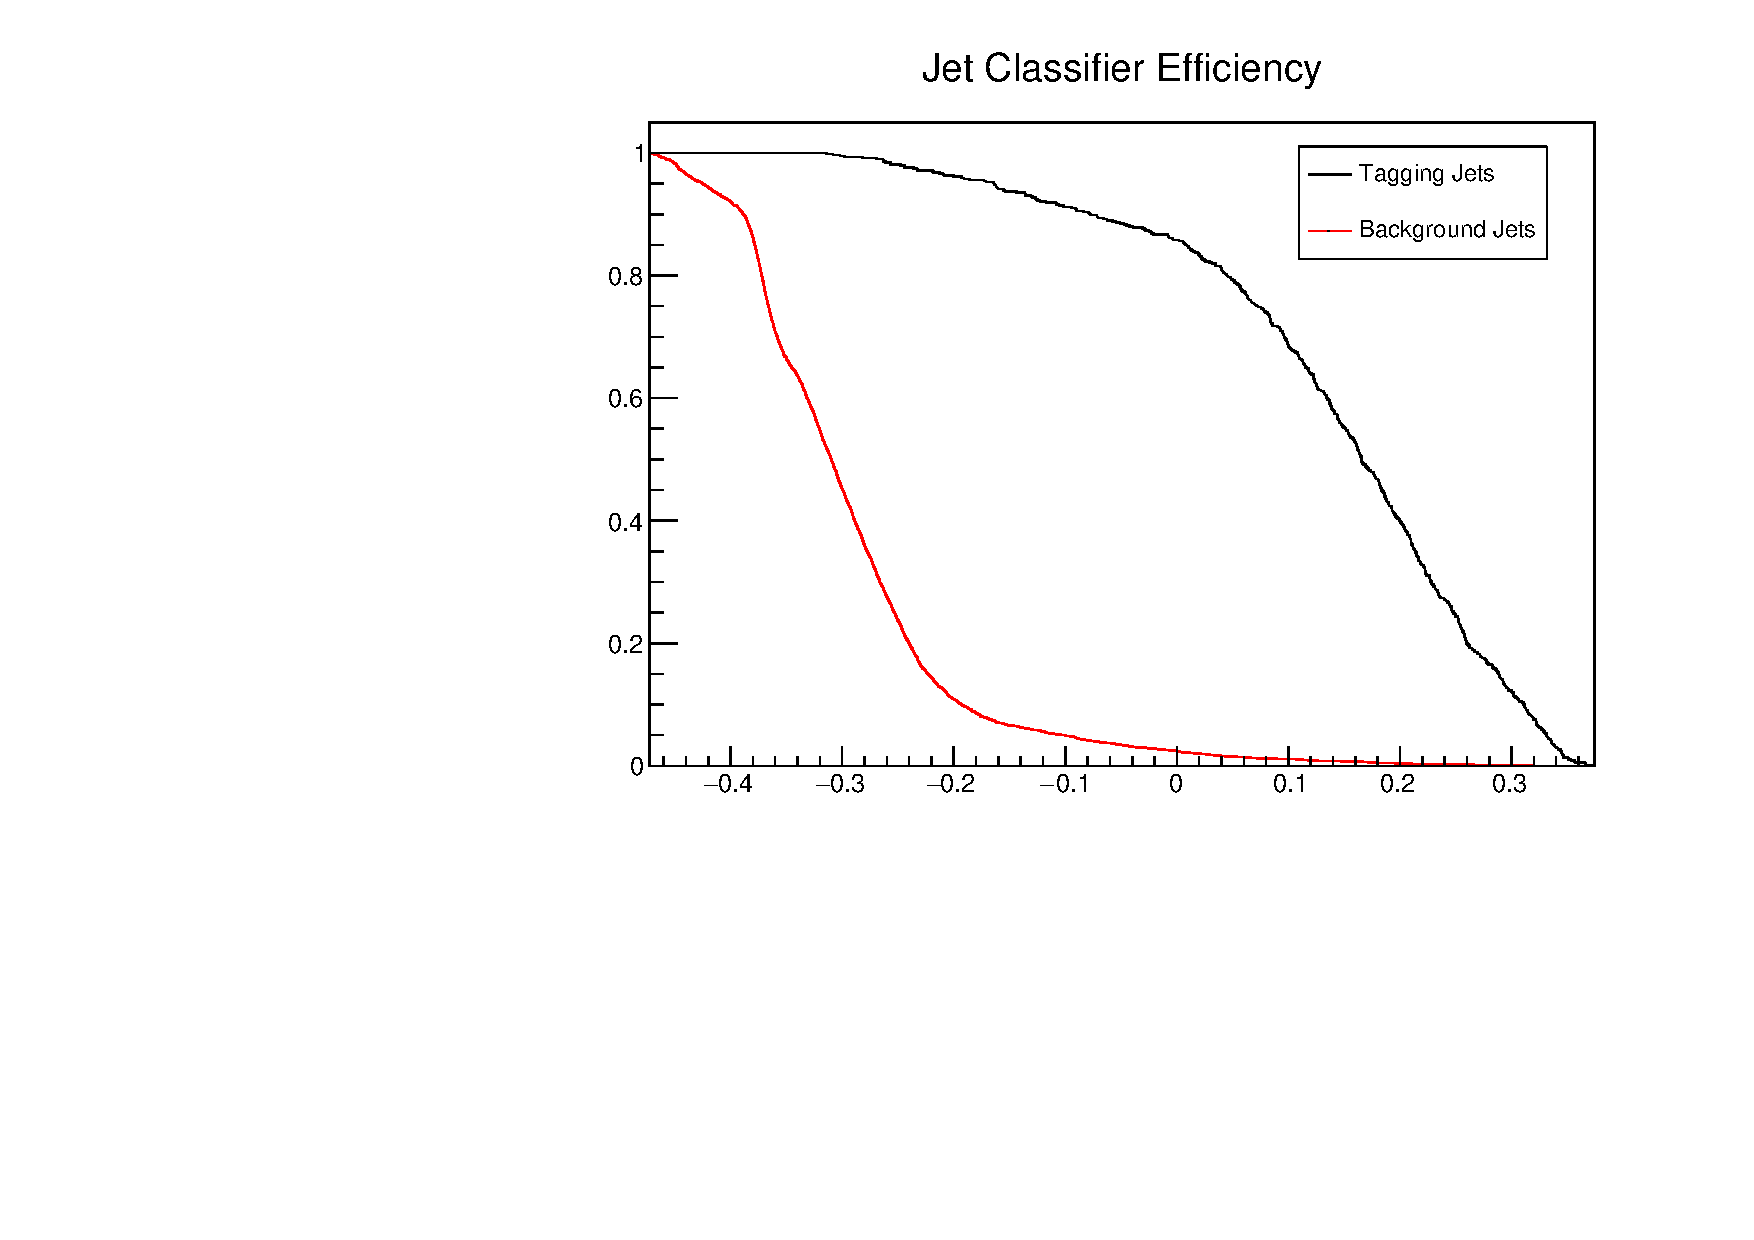
\includegraphics[height=8cm]{images/JetClassifierEff}
\caption{The fraction of jets that are accepted as a function of the cutoff on the BDT response. Since the accepting efficiency decreases much more rapidly for the pileup jets, one can choose a cutoff that rejects most pileup jets while still accepting most tagging jets.}
\label{fig:jetbdteff}
\end{figure}
In order to use the jet classifier once it has been trained, one must choose a cutoff for the classifier response. Jets that score higher than the cutoff are considered tagging jets, and jets scoring lower are considered pileup. Based on the efficiency functions in figure \ref{fig:jetbdteff}, one can choose the cutoff such that $eff_{signal} = 1 - eff_{background}$, which gives a reasonable cutoff in terms of maximizing signal acceptance while minimizing background acceptance. For the jet BDT classifier, this value of the cutoff was -0.144. 

\subsection{Event Classifier}
Selecting events that have two opposite-hemisphere tagging jets (as determined by the tagging jet classifier) eliminates many background events. However, we would like to eliminate even more $t\bar{t}$, $W+3Jets$, and $W+4Jets$ events before calculating the invariant mass spectrum. This can be done with an additional classifier on the events as a whole. By identifying variables that are significantly different between WW scattering events and the types of background events, a classifier can be created that rejects more background than signal, thus increasing the signal-to-noise ratio. \par
For the event classifier, the following variables were used:
\begin{itemize}
\item Hadronic Jet $|\eta|$
\item Hadronic Jet $p_t$
\item Hadronic Jet mass
\item Missing transverse energy magnitude
\item Tagging jet pair invariant mass
\item Lepton $|\eta|$
\item Lepton $p_t$
\end{itemize}
Using sets of 100,000 WW scattering, $t\bar{t}$, $W+3Jets$, and $W+4Jets$ events processed by Pythia and Delphes, I partitioned each of the events files in the following way:
\begin{itemize}
\item 0 - 999: Jet classifier training set (WW scattering only)
\item 1000 - 9999: Event classifier training/testing set
\item 10000 - 100000: Reconstruction
\end{itemize}
After training the jet classifier on the first 1,000 WW scattering events, I trained the event classifier on the events from 1000 - 9999, including only events that had all the required components (lepton, hadronic jet, and two tagging jets that pass the jet classifier). WW scattering events were the signal, and $t\bar{t}$, $W+3Jets$, and $W+4Jets$ were the background. The performance of the event classifier is shown in figure \ref{fig:eventldeff}.
\begin{figure}
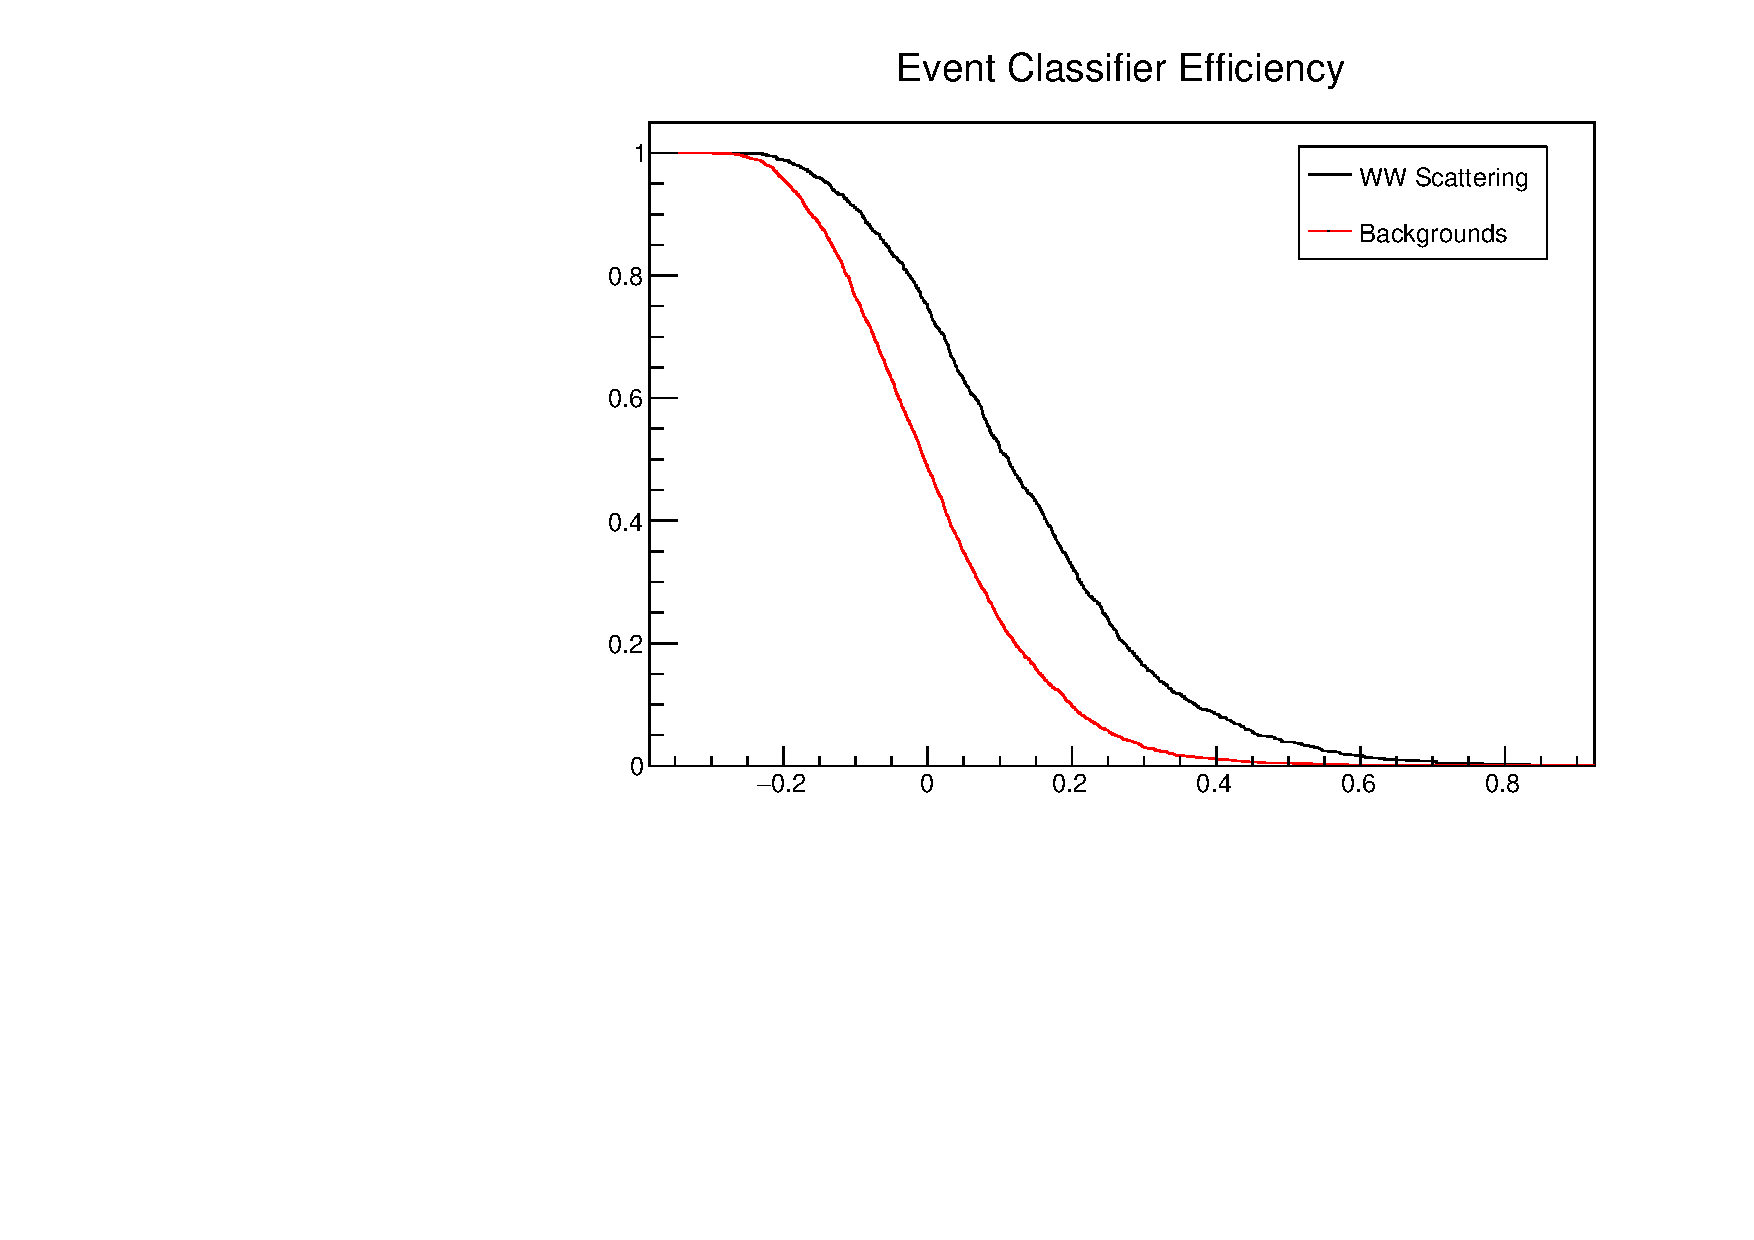
\includegraphics[height=8cm]{images/EventClassifierEff}
\caption{Efficiency of the event classifier for signal and background, as a function of the cutoff. The event classifier is less effective at distinguishing WW scattering events from background than the jet classifier is at distinguishing tagging jets from pileup, as seen from the fact that the signal and background efficiency curves are close together. The event classifier has to reject a large number of signal events in order to significantly reduce the background.}
\label{fig:eventldeff}
\end{figure}
After training the event classifier, I calculated invariant mass spectra for the remaining 90,000 events, first filtering out any events that didn't have the required components, or didn't pass the event classifier. The numbers of events of each type that made it through the event selection process are shown in table \ref{tab:eventselection}

\begin{table}[]
\centering
\resizebox{\textwidth}{!}{\begin{tabular}{llllll}
Type & Missing tag jets & Other missing particle(s) & Failed event classifier & Bad reconstruction & Good events\\
SM $W^+W^-$ & 9781 & 73160 & 1420 & 3169 & 2462 \\
$t\bar{t}$ & 26486 & 57305 & 2822 & 1608 & 1779\\
$W+3Jets$ & 24610 & 32668 & 28801 & 2099 & 1822\\
$W+4Jets$ & 48299 & 33003 & 4653 & 2167 & 1878 \\
$W^{+}W^{-}, \Lambda = 500$ GeV & 18973 & 52811 & 3042 & 8121 & 7053\\
$W^{+}W^{-}, \Lambda = 466$ GeV & 17594 & 53109 & 2870 & 8495 & 7932\\
$W^{+}W^{-}, \Lambda = 433$ GeV & 15860 & 53149 & 2626 & 9355 & 9010\\
$W^{+}W^{-}, \Lambda = 400$ GeV & 6240 & 73648 & 1080 & 4489 & 4543
\end{tabular}}
\caption{The number of events (out of 90,000 starting events) that make it through each step of the event classification.}
\label{tab:eventselection}
\end{table}

\begin{figure}
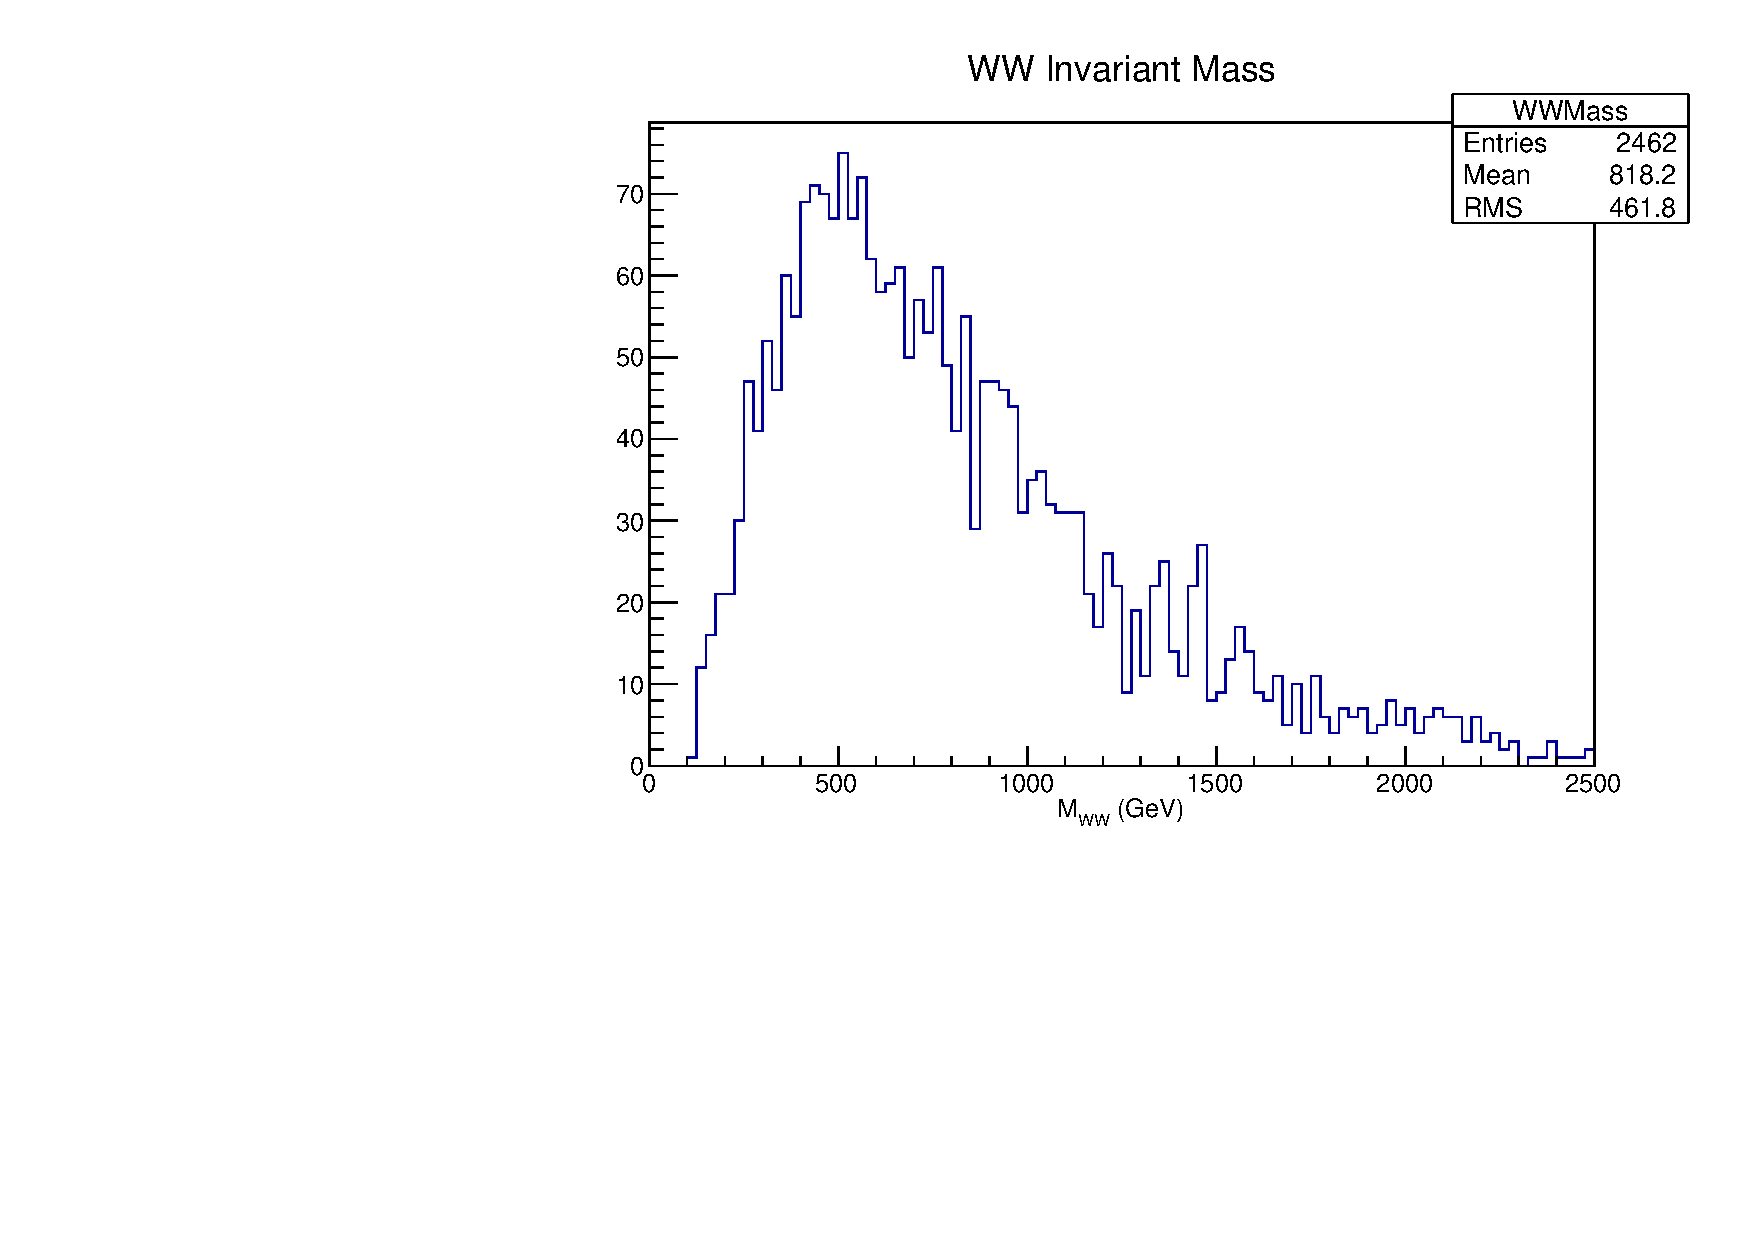
\includegraphics[height=8cm]{images/SMWWSpectrum}
\caption{Histogram of the invariant mass of the $W^{+}W^{-}$ boson pair in semi-leptonic WW scattering, with events filtered by the event classifier. The invariant mass of the boson pair is calculated by solving for the four-vector of the neutrino using equation \ref{eq:pzsol}, with negative discriminants resolved by equation \ref{eq:metfit}.}
\label{fig:smwwspectrum}
\end{figure}
\section{Hypothesis Testing}
Once invariant mass spectra have been obtained for standard model W+W- scattering, the three background processes, and beyond-the-standard-model $W^+W^-$ scattering, the next step is to test whether the new physics theories could be ruled out by the phase-II LHC. One needs a way of checking whether the difference in the observed WW scattering spectrum between the Standard Model and the new theories is statistically significant, in the presence of the background processes. To do this, I use a \textit{profile likelihood test}. The profile likelihood test takes a distribution and a set of data points, and checks whether those points are likely to have been drawn from that distribution. It does this by dividing the data points into bins along the x-axis, and computing the probability of each point, assuming a Poisson distribution with mean determined by the value of the true distribution in each bin.\cite{ranucci} The likelihood of the observed dataset is the product of the likelihoods in each bin:
\begin{equation} \label{eq:likelihood}
P(n_i, \theta, \mu) = \prod_{i}{\frac{(\mu s_i + (1 - \mu)s^0_i + b_i^{n_i} e^{-(\mu s_i + (1 - \mu)s^0_i + b_i)}}{n_i!}}
\end{equation}
where $s_i$ is the expected number of events in bin $i$ under the alternate model (in this case the effective operator theories), $s^0_i$ is the expected number under the null model (the Standard Model in this case), $n_i$ is the observed number of events, $\mu$ is the \textit{parameter of interest} of the model, and $\theta$ is the set of all other parameters of the model (such as fit parameters). The parameter $\mu$ varies the model between the null and alternate hypotheses - if $\mu$ is zero, equation \ref{eq:likelihood} reduces to the standard model invariant mass spectrum with background. If $\mu$ is one, it reduces to the effective operator mass spectrum with background. The profile likelihood is then defined as:
\begin{equation} \label{eq:proflikelihood}
\lambda(n_i) = \frac{P(n_i, \hat{\theta}, \mu = 1)}{P(n_i, \hat{\theta}, \mu = 0)}
\end{equation}
where $\hat{\theta}$ is the value of $\theta$ that maximizes P for each value of $\mu$. The $\theta$ parameters are called \textit{nuissance parameters} because we are not attempting to set constraints on their values. According to Wilks' theorem, the quantity $t = -2ln\lambda(\mu)$ is distributed according to a $\chi^2$ distribution with one degree of freedom, which allows computation of the p-value of the observed measurements. \par
To use the profile likelihood test for testing the effective operator theories, I created fits of all of the invariant mass spectra. I assumed that each spectrum could be fit with an exponential function representing background events plus a Gaussian function representing the signal at higher energies:
\begin{equation} \label{eq:mwwfit}
P(M_{WW}) = Ae^{-\alpha M_{WW}} + Be^{\frac{-(M_{WW} - \mu)^2}{2\sigma^2}}
\end{equation}
This fit function was chosen under the assumption that some background events would be accepted by the event classifier, meaning that all invariant mass spectra would have both signal and background contributions.
\begin{figure}
	\begin{subfigure}[b]{8cm}
    	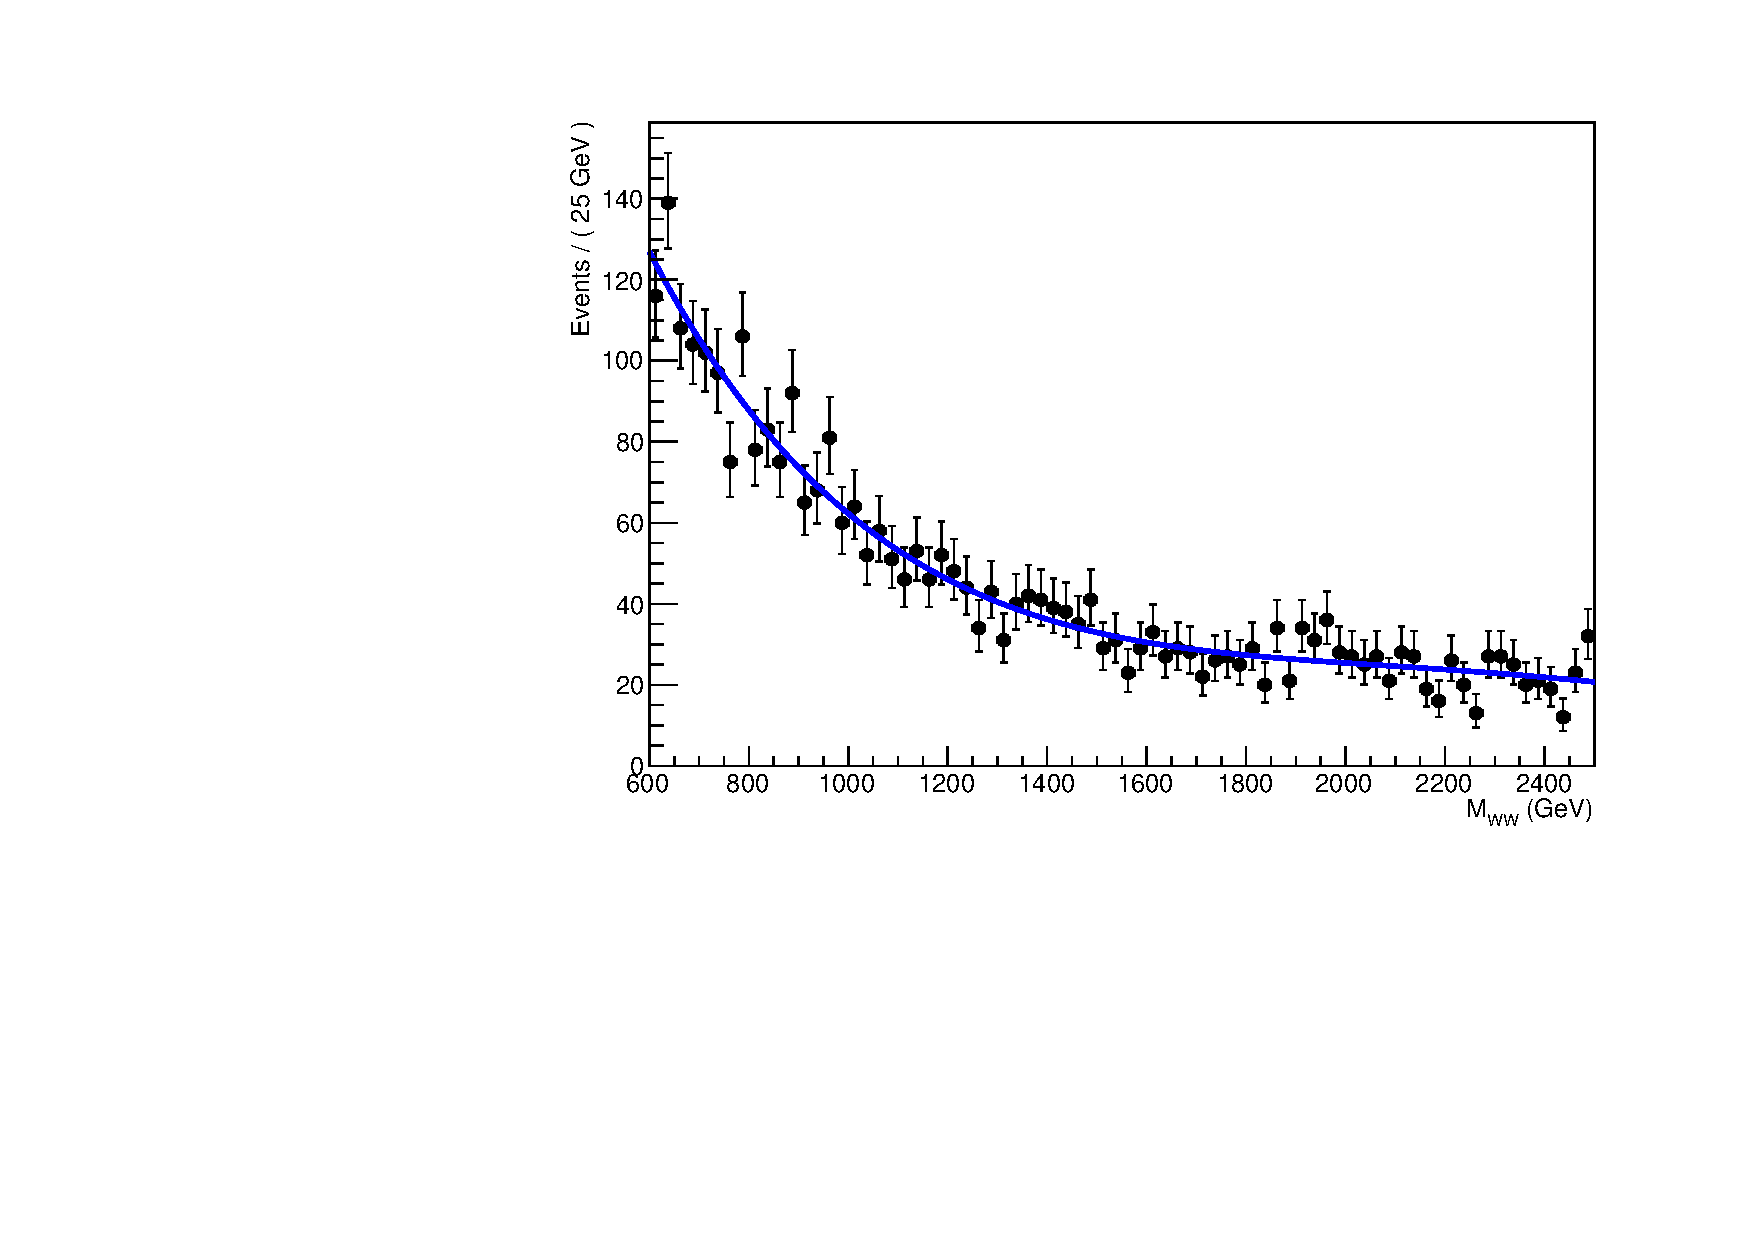
\includegraphics[width=\textwidth]{images/Eff400fit}
        \subcaption{$\Lambda = 500$ GeV}
    \end{subfigure}
    \begin{subfigure}[b]{8cm}
    	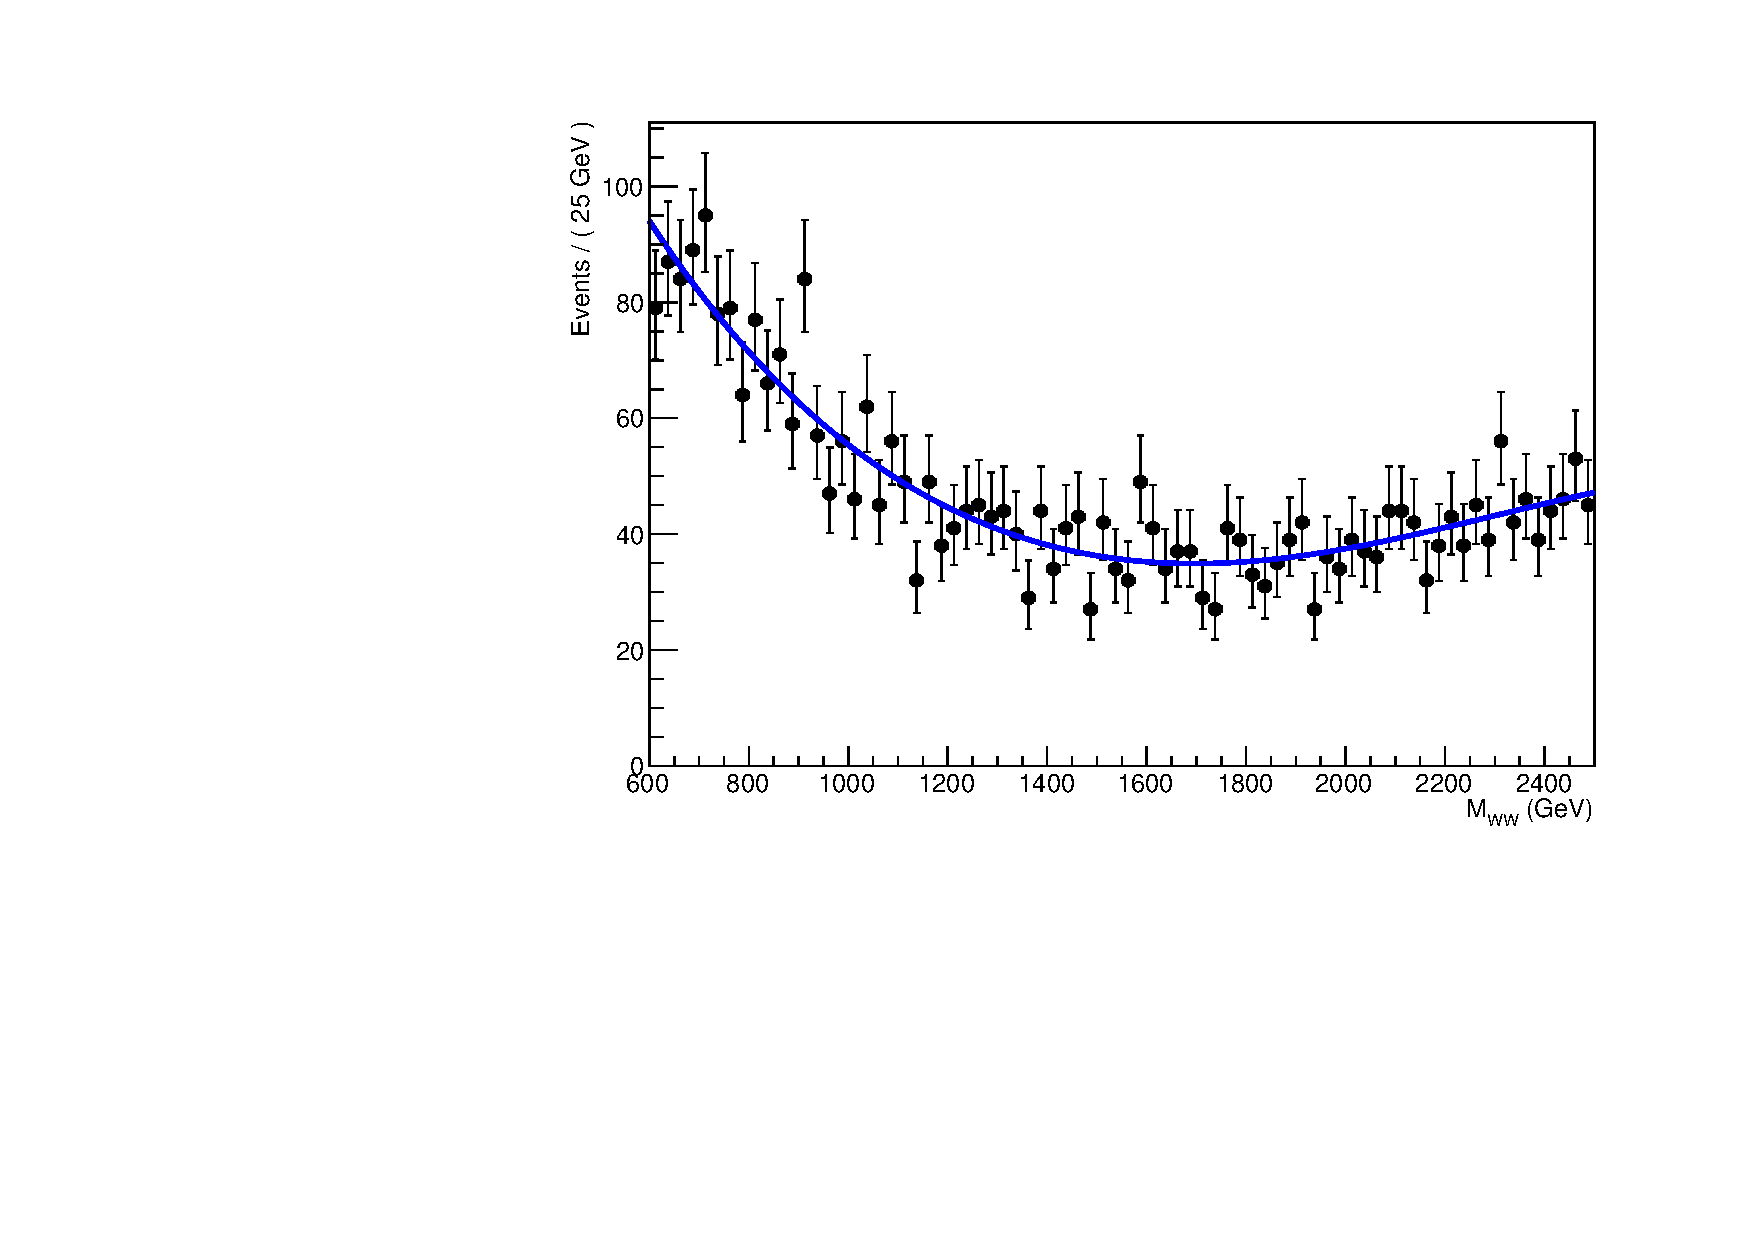
\includegraphics[width=\textwidth]{images/Eff533fit}
        \subcaption{$\Lambda = 433$ GeV}
    \end{subfigure}
\caption{The invariant mass spectra of the W boson pairs in WW scattering with effective operator contributions (equation \ref{eq:effectivelagrangian}) for two different values of the scale $\Lambda$, with fits to equation \ref{eq:mwwfit}. The effective operator contributions are more apparent in (b) because the scale of new physics is lower, causing effects at lower energies.}
\label{fig:spectrumfits}
\end{figure}
Figure \ref{fig:spectrumfits} shows invariant mass spectra (after detector simulation and event selection) of two of the effective operator theories with fits to \ref{eq:mwwfit}.
I then created the combined model by adding the models of the spectra according to their cross-sections:
\begin{equation}
P_{combined}(M_{WW}, \mu) = W_{t\bar{t}}P_{t\bar{t}} + W_{W+3j}P_{W+3j} + W_{W+4j}P_{W+4j} + W_{W^+W^-}[\mu P_{SM} + (1-\mu)P_{eff}]
\end{equation}
where $W_{t\bar{t}}$, $W_{W+3j}$, $W_{W+4j}$, and $W_{W^+W^-}$ are set such that they are proportional to the relative cross-sections and add up to one. For $t\bar{t}$, this is given by:
\begin{equation}
W_{t\bar{t}} = \frac{\sigma_{t\bar{t}}}{\sigma_{t\bar{t}} + \sigma_{W+3j} + \sigma_{W+4j} + \sigma_{W^+W^-}}
\end{equation}
The $W^+W^-$ scattering weight is kept fixed regardless of whether it is governed by the effective operator theories or the standard model (this is determined by the value of $\mu$). 
\begin{figure}
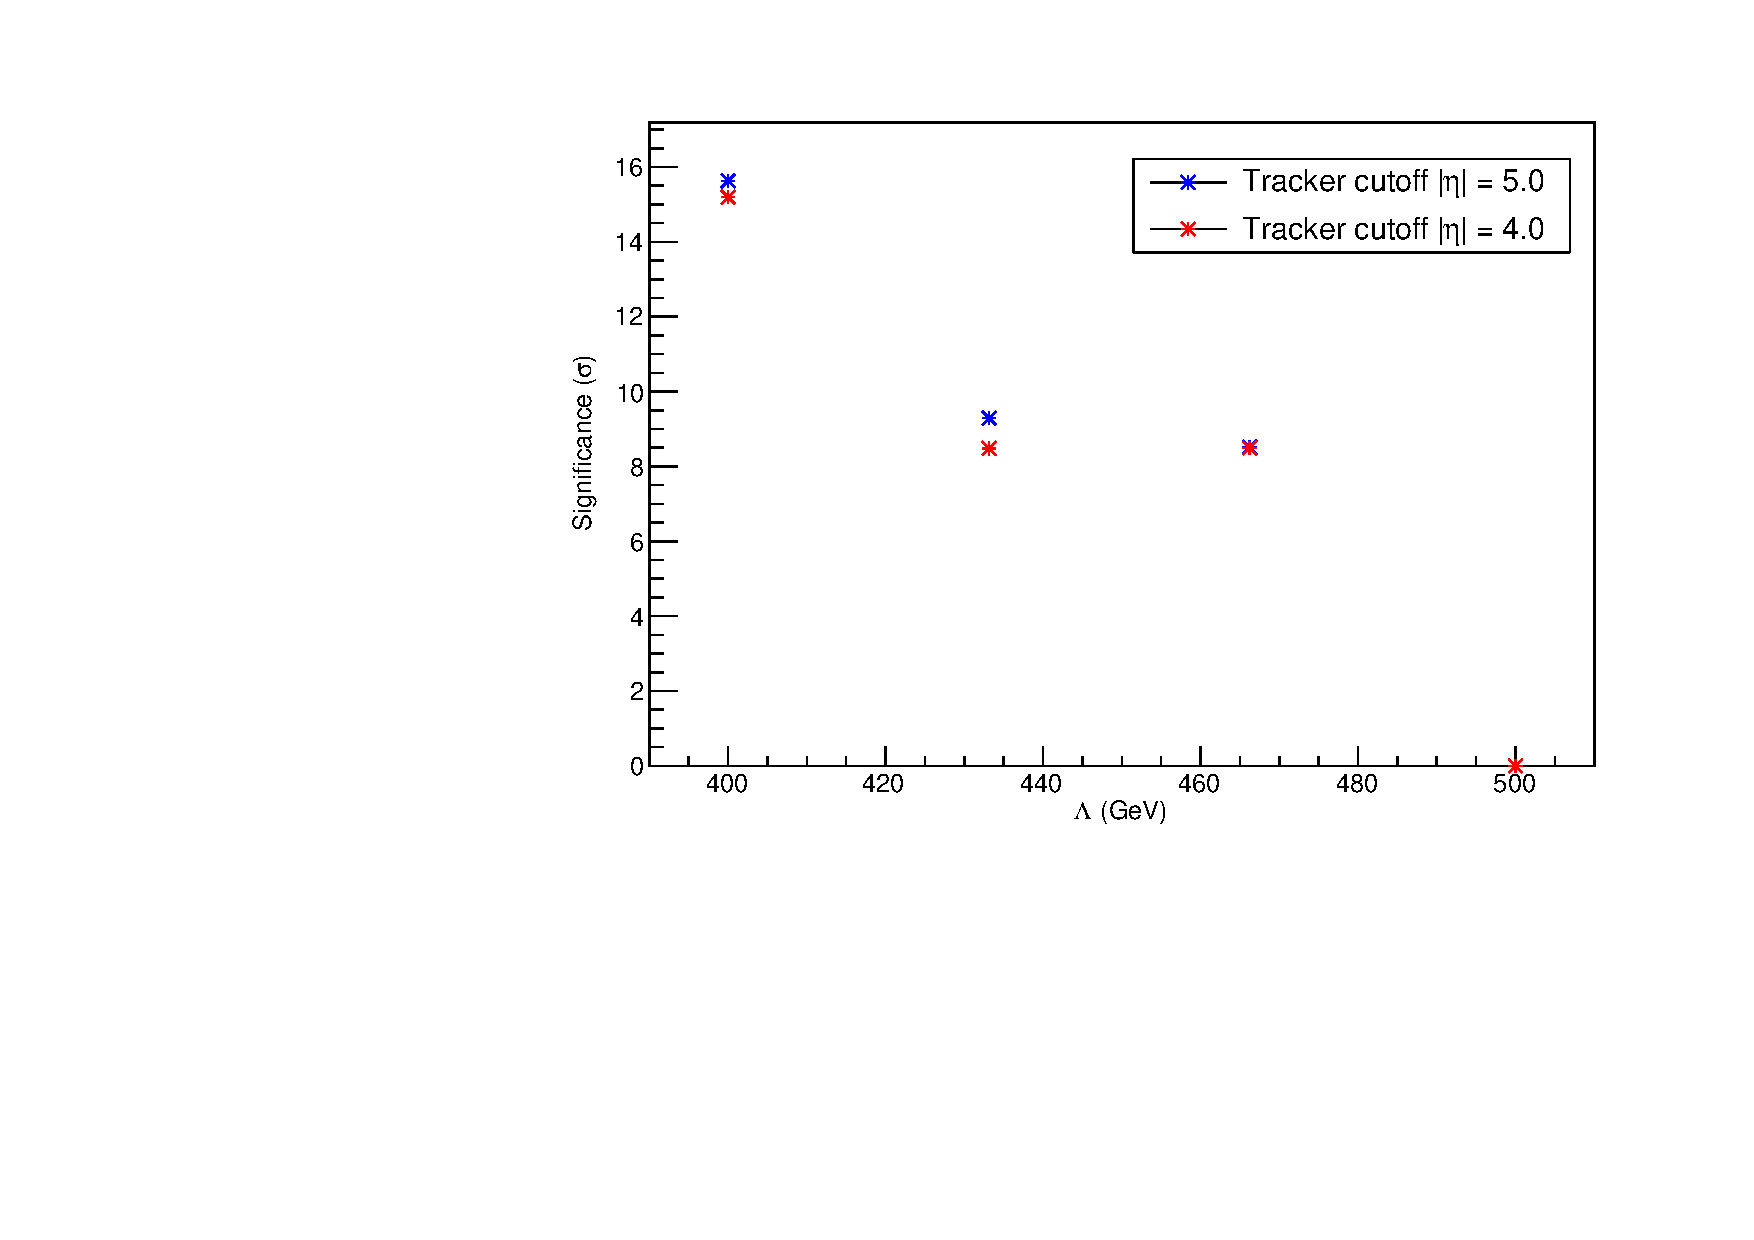
\includegraphics[width=\linewidth]{images/SignificancePlot}
\caption{The profile likelihood significance of a simulated Standard Model WW scattering dataset under the effective operator theory. The significance is slightly lower when tracker coverage for jets is reduced to the region $|\eta| < 4.0$.}
\label{fig:SignificancePlot}
\end{figure}
The profile likelihood test, as implemented in the RooStats package \cite{roostats} creates a sample dataset according to the model under the null hypothesis ($\mu = 0$) and checks the value of the profile likelihood statistic (equation \ref{eq:proflikelihood}) with $\mu = 1$ (the alternate hypothesis). The probability of that value of the profile likelihood can then be estimated from Wilks' theorem, giving the significance of the observed dataset in Gaussian standard deviations. In this case, I set the size of the generated dataset according to:
\begin{equation}
N = L_{int}\sigma_{W^+W^-}
\end{equation}
where $L_{int}$ is the integrated luminosity of the LHC over the time period during which data is being collected. I estimated the integrated luminosity at $10 fb^{-1}$, which is probably a very low estimate. Therefore, $N$ is an estimate of the number of total leptonic WW scattering events that should be observed during the operation of the LHC. \par
The significance of the deviation of the effective operator mass spectra from the Standard Model is shown in figure \ref{fig:SignificancePlot}, as a function of the scale of new physics $\Lambda$. 
If $3\sigma$ certainty is desired, we might be able to rule out the effective operator theories for values of $\Lambda$ below $470$ GeV. Figure \ref{fig:SignificancePlot} shows these significance values for two different values of the tracker cutoff, $|\eta| < 4.0$ and $|\eta| < 5.0$. For each cutoff value, I erased the JVF information for jets with $|\eta|$ greater than the cutoff in all training and experiment sets, and re-ran the analysis from scratch. Decreasing the tracker coverage seems to have some effect on the significance for lower values of $\Lambda$. 
\chapter{Conclusion}
Using simulated WW scattering events under the Standard Model and effective operator theories, I was able to create an estimate of which values of $\Lambda$, the effective operator scale, could be ruled out by experiments at the high-luminosity phase-II LHC. Using machine learning classifiers to detect the components of leptonic WW scattering events, I was able to filter out some events from background processes like $t\bar{t}$, $W+3j$, and $W+4j$ and to reject tagging jets from pileup vertices. I also attempted to simulate realistic detector performance at the phase-II ATLAS detector by using Delphes to apply Gaussian "smearing" to the particle energies and momenta, with the variance of the smearing determined by predictions that have been made about how the phase-II detectors will perform.  
\appendix
\nocite{*}

\begin{thebibliography}{999}
\bibitem{kilian2014}W. Kilian, T. Ohl, J. Reuter, and M. Sekulla.
Phys.\ Rev.\ D {\bf 91}, 096007 (2015).
\bibitem{khachatryan2015}V. Khachatryan \textit{et al.}, "Study of Vector Boson Scattering and Search For New Physics in Events With Two Same-sign Leptons and Two Jets",
Phys.\ Rev.\ Lett.\ {\bf 114}, 051801 (2015).
\bibitem{fabbrichesi2015}M. Fabbrichesi, M. Pinamonte, A. Tonero, A. Urbano, "Vector boson scattering at the LHC: A study of the WW -> WW channels with the Warsaw Cut", 2015.
\bibitem{atlasnote2012}The ATLAS Collaboration, "Studies of Vector Boson Scattering With an Upgraded ATLAS Detector at a High-Luminosity LHC", 2012. 
\bibitem{yanou2015}Y. Cui, Z. Han, "New Light on WW Scattering at the LHC With W Jet Tagging", Phys.\ Rev.\ D {\bf 89}, 015019 (2014).
\bibitem{moreno2009}M. Moreno, R. Moles, V. Lacuesta, "Top Quark Mass Reconstruction in the semi-leptonic channel using the Global Chi-squared algorithm", 2009.
\bibitem{delphes}J. de Favereau, C. Delaere, \textit{et al.}, "DELPHES 3: a modular framework for fast simulation of a generic collider experiment", Journal of High-Energy Physics, 2014.
\bibitem{ATLASElectronRes}The ATLAS Collaboration, "Performance assumptions for an upgraded ATLAS detector at a High-Luminosity LHC", 2013.
\bibitem{ATLASMuonRes}The ATLAS Collaboration, "Performance assumptions based on full simulation of an upgraded ATLAS detector at a High-Luminosity LHC", 2013.
\bibitem{ATLASJVF}"Pile-up subtraction and suppression for jets in ATLAS", The ATLAS Collaboration, 2013.
\bibitem{BDT}Friedman, Jerome H. "Greedy Function Approximation: A Gradient Boosting Machine", The Annals of Statistics, Vol 29. No. 5 (2001).
\bibitem{nik}Garner, Niklas. "Vector Boson Scattering at the High-Luminosity Large Hadron Collider", 2015.
\bibitem{ranucci}Ranucci, Gioacchino. "The profile likelihood ratio and the look elsewhere effect in high-energy physics." Nucl.Instrum.Meth. A661 (2012) 77-85.
\bibitem{vbfnlo1}Baglio, J., Bellm, J, \textit{et al.}, "Release note - VBFNLO 27.0", 2014.
\bibitem{vbfnlo2}Arnold, K., Bahr M., \textit{et al.}, "VBFNLO: A parton level Monte Carlo for processes with electroweak bosons", 2009.
\bibitem{smoverview}Herrero, M. "The Standard Model". NATO Sci.Ser.C 534 (1999) 1-59 hep-ph/9812242 FTUAM-98-25
\bibitem{higgsdiscovery}The ATLAS Collaboration, "Observation of a new particle in the search for the Standard Model Higgs boson with the ATLAS detector at the LHC", Phys. Lett. B 1, 716 (2012).
\bibitem{tong}Tong, D. "Quantum Field Theory". University of Cambridge, 2007.
\bibitem{LHC2008}The ATLAS Collaboration, "The ATLAS Experiment at the CERN Large Hadron Collider", JINST 3 S08003 (2008).
\bibitem{ATLASDiagram}The ATLAS Collaboration, "ATLAS Overview and Main Results", 2013.
\bibitem{MonteCarloHowTo}Papaefstathiou, A., "How-to: Write a parton-level Monte Carlo event generator", arXiv:1412.4677 (2014).
\bibitem{roostats}Moneta, Lorenzo \textit{et al.}, "The RooStats Project", PoS ACAT2010 (2010) 057 arXiv:1009.1003 [physics.data-an]
\bibitem{atlasupgrade}The ATLAS Collaboration, "Physics at a High-Luminosity LHC with ATLAS", 2013.
\bibitem{madgraph}Alwall, J., \textit{et al.}, "The automated computation of tree-level and next-to-leading order differential cross sections, and their matching to parton shower simulations", 2014.
\bibitem{pythia}Sjostrand, T. "PYTHIA 6.4 Physics and Manual", 2006.
\end{thebibliography}
\end{document}
